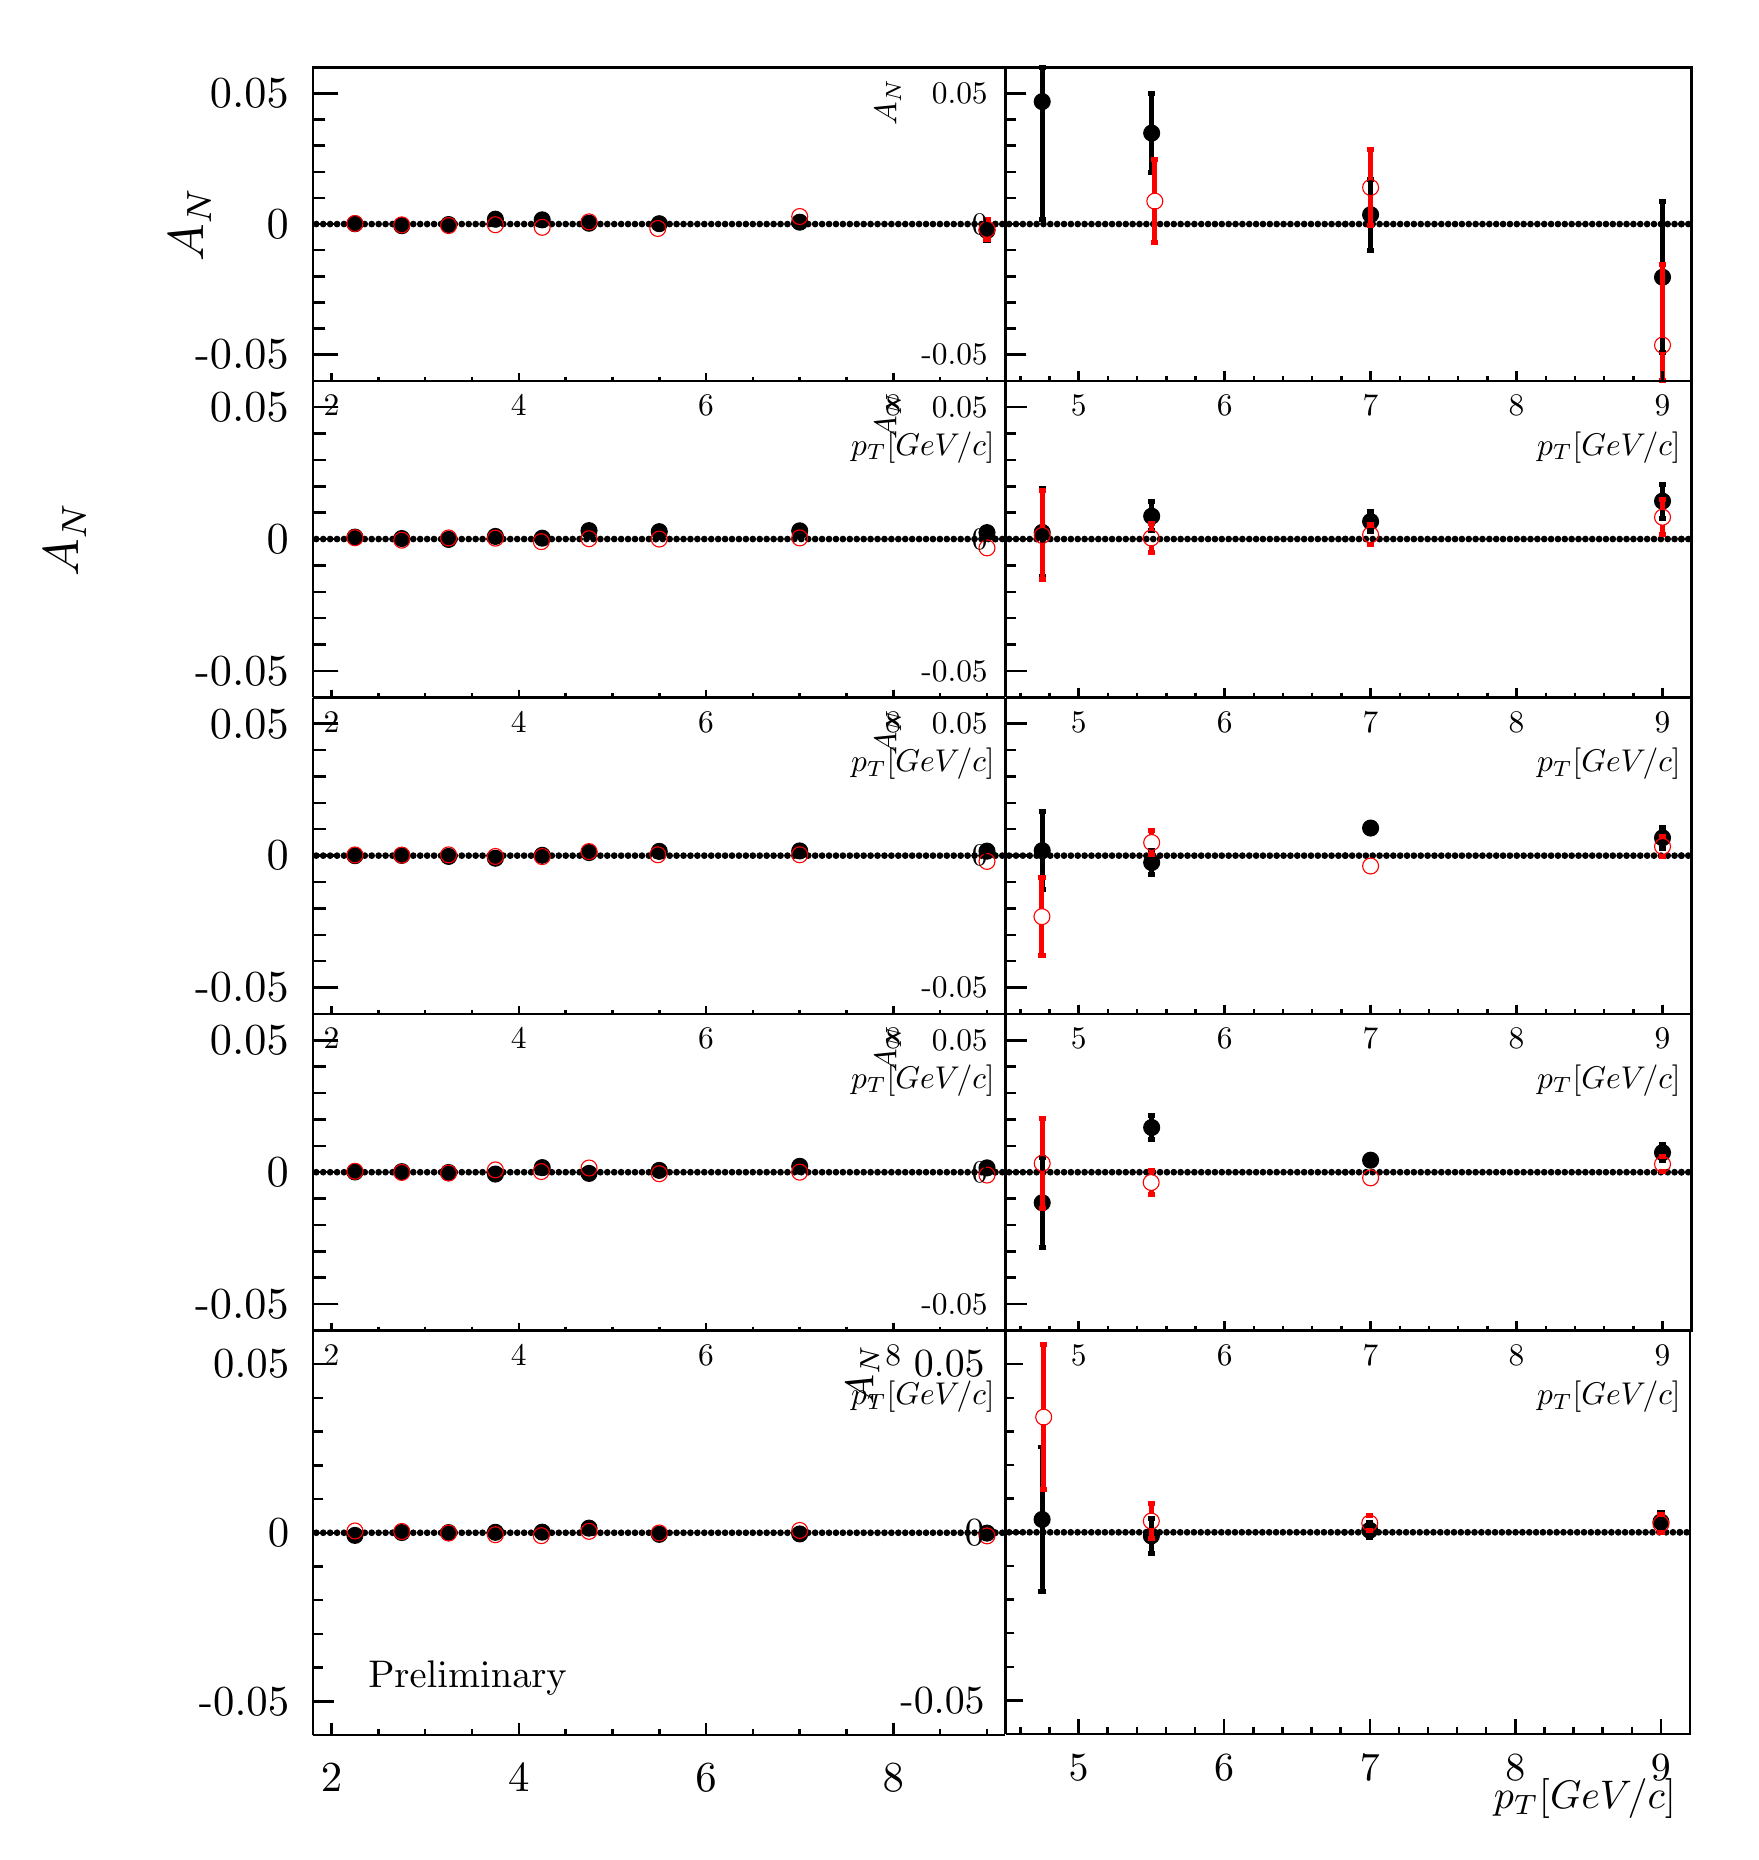
\begin{tikzpicture}
\pgfdeclareplotmark{cross} {
\pgfpathmoveto{\pgfpoint{-0.3\pgfplotmarksize}{\pgfplotmarksize}}
\pgfpathlineto{\pgfpoint{+0.3\pgfplotmarksize}{\pgfplotmarksize}}
\pgfpathlineto{\pgfpoint{+0.3\pgfplotmarksize}{0.3\pgfplotmarksize}}
\pgfpathlineto{\pgfpoint{+1\pgfplotmarksize}{0.3\pgfplotmarksize}}
\pgfpathlineto{\pgfpoint{+1\pgfplotmarksize}{-0.3\pgfplotmarksize}}
\pgfpathlineto{\pgfpoint{+0.3\pgfplotmarksize}{-0.3\pgfplotmarksize}}
\pgfpathlineto{\pgfpoint{+0.3\pgfplotmarksize}{-1.\pgfplotmarksize}}
\pgfpathlineto{\pgfpoint{-0.3\pgfplotmarksize}{-1.\pgfplotmarksize}}
\pgfpathlineto{\pgfpoint{-0.3\pgfplotmarksize}{-0.3\pgfplotmarksize}}
\pgfpathlineto{\pgfpoint{-1.\pgfplotmarksize}{-0.3\pgfplotmarksize}}
\pgfpathlineto{\pgfpoint{-1.\pgfplotmarksize}{0.3\pgfplotmarksize}}
\pgfpathlineto{\pgfpoint{-0.3\pgfplotmarksize}{0.3\pgfplotmarksize}}
\pgfpathclose
\pgfusepathqstroke
}
\pgfdeclareplotmark{cross*} {
\pgfpathmoveto{\pgfpoint{-0.3\pgfplotmarksize}{\pgfplotmarksize}}
\pgfpathlineto{\pgfpoint{+0.3\pgfplotmarksize}{\pgfplotmarksize}}
\pgfpathlineto{\pgfpoint{+0.3\pgfplotmarksize}{0.3\pgfplotmarksize}}
\pgfpathlineto{\pgfpoint{+1\pgfplotmarksize}{0.3\pgfplotmarksize}}
\pgfpathlineto{\pgfpoint{+1\pgfplotmarksize}{-0.3\pgfplotmarksize}}
\pgfpathlineto{\pgfpoint{+0.3\pgfplotmarksize}{-0.3\pgfplotmarksize}}
\pgfpathlineto{\pgfpoint{+0.3\pgfplotmarksize}{-1.\pgfplotmarksize}}
\pgfpathlineto{\pgfpoint{-0.3\pgfplotmarksize}{-1.\pgfplotmarksize}}
\pgfpathlineto{\pgfpoint{-0.3\pgfplotmarksize}{-0.3\pgfplotmarksize}}
\pgfpathlineto{\pgfpoint{-1.\pgfplotmarksize}{-0.3\pgfplotmarksize}}
\pgfpathlineto{\pgfpoint{-1.\pgfplotmarksize}{0.3\pgfplotmarksize}}
\pgfpathlineto{\pgfpoint{-0.3\pgfplotmarksize}{0.3\pgfplotmarksize}}
\pgfpathclose
\pgfusepathqfillstroke
}
\pgfdeclareplotmark{newstar} {
\pgfpathmoveto{\pgfqpoint{0pt}{\pgfplotmarksize}}
\pgfpathlineto{\pgfqpointpolar{44}{0.5\pgfplotmarksize}}
\pgfpathlineto{\pgfqpointpolar{18}{\pgfplotmarksize}}
\pgfpathlineto{\pgfqpointpolar{-20}{0.5\pgfplotmarksize}}
\pgfpathlineto{\pgfqpointpolar{-54}{\pgfplotmarksize}}
\pgfpathlineto{\pgfqpointpolar{-90}{0.5\pgfplotmarksize}}
\pgfpathlineto{\pgfqpointpolar{234}{\pgfplotmarksize}}
\pgfpathlineto{\pgfqpointpolar{198}{0.5\pgfplotmarksize}}
\pgfpathlineto{\pgfqpointpolar{162}{\pgfplotmarksize}}
\pgfpathlineto{\pgfqpointpolar{134}{0.5\pgfplotmarksize}}
\pgfpathclose
\pgfusepathqstroke
}
\pgfdeclareplotmark{newstar*} {
\pgfpathmoveto{\pgfqpoint{0pt}{\pgfplotmarksize}}
\pgfpathlineto{\pgfqpointpolar{44}{0.5\pgfplotmarksize}}
\pgfpathlineto{\pgfqpointpolar{18}{\pgfplotmarksize}}
\pgfpathlineto{\pgfqpointpolar{-20}{0.5\pgfplotmarksize}}
\pgfpathlineto{\pgfqpointpolar{-54}{\pgfplotmarksize}}
\pgfpathlineto{\pgfqpointpolar{-90}{0.5\pgfplotmarksize}}
\pgfpathlineto{\pgfqpointpolar{234}{\pgfplotmarksize}}
\pgfpathlineto{\pgfqpointpolar{198}{0.5\pgfplotmarksize}}
\pgfpathlineto{\pgfqpointpolar{162}{\pgfplotmarksize}}
\pgfpathlineto{\pgfqpointpolar{134}{0.5\pgfplotmarksize}}
\pgfpathclose
\pgfusepathqfillstroke
}
\definecolor{c}{rgb}{0.999,0.999,0.999};
\draw [color=c, fill=c] (0,0) rectangle (20,22.8439);
\definecolor{c}{rgb}{0,0,0};
\draw [anchor=base west] (0.2,0.228439) node[scale=1.12974, color=c, rotate=0]{Tue Oct  6 03:21:55 2020};
\definecolor{c}{rgb}{1,1,1};
\draw [color=c, fill=c] (0,0) rectangle (10.8,6.30492);
\draw [color=c, fill=c] (2,1.16758) rectangle (10.8,6.30492);
\definecolor{c}{rgb}{0,0,0};
\draw [c,line width=0.9] (2,1.16758) -- (2,6.30492) -- (10.8,6.30492) -- (10.8,1.16758) -- (2,1.16758);
\definecolor{c}{rgb}{1,1,1};
\draw [color=c, fill=c] (2,1.16758) rectangle (10.8,6.30492);
\definecolor{c}{rgb}{0,0,0};
\draw [c,line width=0.9] (2,1.16758) -- (2,6.30492) -- (10.8,6.30492) -- (10.8,1.16758) -- (2,1.16758);
\foreach \P in
 {(2.044,3.73625),(2.132,3.73625),(2.22,3.73625),(2.308,3.73625),(2.396,3.73625),(2.484,3.73625),(2.572,3.73625),(2.66,3.73625),(2.748,3.73625),(2.836,3.73625),(2.924,3.73625),(3.012,3.73625),(3.1,3.73625),(3.188,3.73625),(3.276,3.73625),(3.364,3.736
25),(3.452,3.73625),(3.54,3.73625),(3.628,3.73625),(3.716,3.73625),(3.804,3.73625),(3.892,3.73625),(3.98,3.73625),(4.068,3.73625),(4.156,3.73625),(4.244,3.73625),(4.332,3.73625),(4.42,3.73625),(4.508,3.73625),(4.596,3.73625),(4.684,3.73625),(4.772,3.
73625),(4.86,3.73625),(4.948,3.73625),(5.036,3.73625),(5.124,3.73625),(5.212,3.73625),(5.3,3.73625),(5.388,3.73625),(5.476,3.73625),(5.564,3.73625),(5.652,3.73625),(5.74,3.73625),(5.828,3.73625),(5.916,3.73625),(6.004,3.73625),(6.092,3.73625),(6.18,3
.73625),(6.268,3.73625),(6.356,3.73625)}{\draw[mark options={color=c,fill=c},mark size=2.402402pt,mark=*,mark size=1pt] plot coordinates {\P};}
\foreach \P in
 {(6.356,3.73625),(6.444,3.73625),(6.532,3.73625),(6.62,3.73625),(6.708,3.73625),(6.796,3.73625),(6.884,3.73625),(6.972,3.73625),(7.06,3.73625),(7.148,3.73625),(7.236,3.73625),(7.324,3.73625),(7.412,3.73625),(7.5,3.73625),(7.588,3.73625),(7.676,3.736
25),(7.764,3.73625),(7.852,3.73625),(7.94,3.73625),(8.028,3.73625),(8.116,3.73625),(8.204,3.73625),(8.292,3.73625),(8.38,3.73625),(8.468,3.73625),(8.556,3.73625),(8.644,3.73625),(8.732,3.73625),(8.82,3.73625),(8.908,3.73625),(8.996,3.73625),(9.084,3.
73625),(9.172,3.73625),(9.26,3.73625),(9.348,3.73625),(9.436,3.73625),(9.524,3.73625),(9.612,3.73625),(9.7,3.73625),(9.788,3.73625),(9.876,3.73625),(9.964,3.73625),(10.052,3.73625),(10.14,3.73625),(10.228,3.73625),(10.316,3.73625),(10.404,3.73625),(1
0.492,3.73625),(10.58,3.73625),(10.668,3.73625)}{\draw[mark options={color=c,fill=c},mark size=2.402402pt,mark=*,mark size=1pt] plot coordinates {\P};}
\foreach \P in {(10.668,3.73625),(10.756,3.73625)}{\draw[mark options={color=c,fill=c},mark size=2.402402pt,mark=*,mark size=1pt] plot coordinates {\P};}
\draw [c,line width=0.9] (2,1.16758) -- (10.8,1.16758);
\draw [c,line width=0.9] (2.23784,1.3217) -- (2.23784,1.16758);
\draw [c,line width=0.9] (2.83243,1.24464) -- (2.83243,1.16758);
\draw [c,line width=0.9] (3.42703,1.24464) -- (3.42703,1.16758);
\draw [c,line width=0.9] (4.02162,1.24464) -- (4.02162,1.16758);
\draw [c,line width=0.9] (4.61622,1.3217) -- (4.61622,1.16758);
\draw [c,line width=0.9] (5.21081,1.24464) -- (5.21081,1.16758);
\draw [c,line width=0.9] (5.80541,1.24464) -- (5.80541,1.16758);
\draw [c,line width=0.9] (6.4,1.24464) -- (6.4,1.16758);
\draw [c,line width=0.9] (6.99459,1.3217) -- (6.99459,1.16758);
\draw [c,line width=0.9] (7.58919,1.24464) -- (7.58919,1.16758);
\draw [c,line width=0.9] (8.18378,1.24464) -- (8.18378,1.16758);
\draw [c,line width=0.9] (8.77838,1.24464) -- (8.77838,1.16758);
\draw [c,line width=0.9] (9.37297,1.3217) -- (9.37297,1.16758);
\draw [c,line width=0.9] (2.23784,1.3217) -- (2.23784,1.16758);
\draw [c,line width=0.9] (9.37297,1.3217) -- (9.37297,1.16758);
\draw [c,line width=0.9] (9.96757,1.24464) -- (9.96757,1.16758);
\draw [c,line width=0.9] (10.5622,1.24464) -- (10.5622,1.16758);
\draw [anchor=base] (2.23784,0.455122) node[scale=1.54445, color=c, rotate=0]{2};
\draw [anchor=base] (4.61622,0.455122) node[scale=1.54445, color=c, rotate=0]{4};
\draw [anchor=base] (6.99459,0.455122) node[scale=1.54445, color=c, rotate=0]{6};
\draw [anchor=base] (9.37297,0.455122) node[scale=1.54445, color=c, rotate=0]{8};
\draw [c,line width=0.9] (2,1.16758) -- (2,6.30492);
\draw [c,line width=0.9] (2.264,1.59569) -- (2,1.59569);
\draw [c,line width=0.9] (2.132,2.0238) -- (2,2.0238);
\draw [c,line width=0.9] (2.132,2.45192) -- (2,2.45192);
\draw [c,line width=0.9] (2.132,2.88003) -- (2,2.88003);
\draw [c,line width=0.9] (2.132,3.30814) -- (2,3.30814);
\draw [c,line width=0.9] (2.264,3.73625) -- (2,3.73625);
\draw [c,line width=0.9] (2.132,4.16436) -- (2,4.16436);
\draw [c,line width=0.9] (2.132,4.59248) -- (2,4.59248);
\draw [c,line width=0.9] (2.132,5.02059) -- (2,5.02059);
\draw [c,line width=0.9] (2.132,5.4487) -- (2,5.4487);
\draw [c,line width=0.9] (2.264,5.87681) -- (2,5.87681);
\draw [c,line width=0.9] (2.264,1.59569) -- (2,1.59569);
\draw [c,line width=0.9] (2.132,1.16758) -- (2,1.16758);
\draw [c,line width=0.9] (2.264,5.87681) -- (2,5.87681);
\draw [c,line width=0.9] (2.132,6.30492) -- (2,6.30492);
\draw [anchor= east] (1.892,1.59569) node[scale=1.54445, color=c, rotate=0]{-0.05};
\draw [anchor= east] (1.892,3.73625) node[scale=1.54445, color=c, rotate=0]{0};
\draw [anchor= east] (1.892,5.87681) node[scale=1.54445, color=c, rotate=0]{0.05};
\foreach \P in {(2.53514,3.7028),(3.12973,3.73944),(3.72432,3.73805),(4.31892,3.74219),(4.91351,3.74398),(5.50811,3.79506),(6.4,3.71641),(8.18378,3.72128),(10.5622,3.73177)}{\draw[mark options={color=c,fill=c},mark size=2.882883pt,mark=*] plot
 coordinates {\P};}
\definecolor{c}{rgb}{1,0,0};
\foreach \P in {(2.53514,3.75907),(3.12973,3.75243),(3.72432,3.73264),(4.31892,3.71144),(4.90173,3.69942),(5.50811,3.75442),(6.4,3.73387),(8.18378,3.76539),(10.5622,3.69685)}{\draw[mark options={color=c,fill=c},mark size=2.882883pt,mark=o] plot
 coordinates {\P};}
\definecolor{c}{rgb}{0,0,0};
\draw [anchor=base west] (2.53215,1.77568) node[scale=1.39001, color=c, rotate=0]{Preliminary};
\draw [c,line width=0.9] (2,1.16758) -- (10.8,1.16758);
\draw [c,line width=0.9] (2.23784,1.3217) -- (2.23784,1.16758);
\draw [c,line width=0.9] (2.83243,1.24464) -- (2.83243,1.16758);
\draw [c,line width=0.9] (3.42703,1.24464) -- (3.42703,1.16758);
\draw [c,line width=0.9] (4.02162,1.24464) -- (4.02162,1.16758);
\draw [c,line width=0.9] (4.61622,1.3217) -- (4.61622,1.16758);
\draw [c,line width=0.9] (5.21081,1.24464) -- (5.21081,1.16758);
\draw [c,line width=0.9] (5.80541,1.24464) -- (5.80541,1.16758);
\draw [c,line width=0.9] (6.4,1.24464) -- (6.4,1.16758);
\draw [c,line width=0.9] (6.99459,1.3217) -- (6.99459,1.16758);
\draw [c,line width=0.9] (7.58919,1.24464) -- (7.58919,1.16758);
\draw [c,line width=0.9] (8.18378,1.24464) -- (8.18378,1.16758);
\draw [c,line width=0.9] (8.77838,1.24464) -- (8.77838,1.16758);
\draw [c,line width=0.9] (9.37297,1.3217) -- (9.37297,1.16758);
\draw [c,line width=0.9] (2.23784,1.3217) -- (2.23784,1.16758);
\draw [c,line width=0.9] (9.37297,1.3217) -- (9.37297,1.16758);
\draw [c,line width=0.9] (9.96757,1.24464) -- (9.96757,1.16758);
\draw [c,line width=0.9] (10.5622,1.24464) -- (10.5622,1.16758);
\draw [c,line width=0.9] (2,1.16758) -- (2,6.30492);
\draw [c,line width=0.9] (2.264,1.59569) -- (2,1.59569);
\draw [c,line width=0.9] (2.132,2.0238) -- (2,2.0238);
\draw [c,line width=0.9] (2.132,2.45192) -- (2,2.45192);
\draw [c,line width=0.9] (2.132,2.88003) -- (2,2.88003);
\draw [c,line width=0.9] (2.132,3.30814) -- (2,3.30814);
\draw [c,line width=0.9] (2.264,3.73625) -- (2,3.73625);
\draw [c,line width=0.9] (2.132,4.16436) -- (2,4.16436);
\draw [c,line width=0.9] (2.132,4.59248) -- (2,4.59248);
\draw [c,line width=0.9] (2.132,5.02059) -- (2,5.02059);
\draw [c,line width=0.9] (2.132,5.4487) -- (2,5.4487);
\draw [c,line width=0.9] (2.264,5.87681) -- (2,5.87681);
\draw [c,line width=0.9] (2.264,1.59569) -- (2,1.59569);
\draw [c,line width=0.9] (2.132,1.16758) -- (2,1.16758);
\draw [c,line width=0.9] (2.264,5.87681) -- (2,5.87681);
\draw [c,line width=0.9] (2.132,6.30492) -- (2,6.30492);
\definecolor{c}{rgb}{1,1,1};
\draw [color=c, fill=c] (0,6.30492) rectangle (10.8,10.3255);
\draw [color=c, fill=c] (2,6.30492) rectangle (10.8,10.3255);
\definecolor{c}{rgb}{0,0,0};
\draw [c,line width=0.9] (2,6.30492) -- (2,10.3255) -- (10.8,10.3255) -- (10.8,6.30492) -- (2,6.30492);
\definecolor{c}{rgb}{1,1,1};
\draw [color=c, fill=c] (2,6.30492) rectangle (10.8,10.3255);
\definecolor{c}{rgb}{0,0,0};
\draw [c,line width=0.9] (2,6.30492) -- (2,10.3255) -- (10.8,10.3255) -- (10.8,6.30492) -- (2,6.30492);
\foreach \P in
 {(2.044,8.31519),(2.132,8.31519),(2.22,8.31519),(2.308,8.31519),(2.396,8.31519),(2.484,8.31519),(2.572,8.31519),(2.66,8.31519),(2.748,8.31519),(2.836,8.31519),(2.924,8.31519),(3.012,8.31519),(3.1,8.31519),(3.188,8.31519),(3.276,8.31519),(3.364,8.315
19),(3.452,8.31519),(3.54,8.31519),(3.628,8.31519),(3.716,8.31519),(3.804,8.31519),(3.892,8.31519),(3.98,8.31519),(4.068,8.31519),(4.156,8.31519),(4.244,8.31519),(4.332,8.31519),(4.42,8.31519),(4.508,8.31519),(4.596,8.31519),(4.684,8.31519),(4.772,8.
31519),(4.86,8.31519),(4.948,8.31519),(5.036,8.31519),(5.124,8.31519),(5.212,8.31519),(5.3,8.31519),(5.388,8.31519),(5.476,8.31519),(5.564,8.31519),(5.652,8.31519),(5.74,8.31519),(5.828,8.31519),(5.916,8.31519),(6.004,8.31519),(6.092,8.31519),(6.18,8
.31519),(6.268,8.31519),(6.356,8.31519)}{\draw[mark options={color=c,fill=c},mark size=2.402402pt,mark=*,mark size=1pt] plot coordinates {\P};}
\foreach \P in
 {(6.356,8.31519),(6.444,8.31519),(6.532,8.31519),(6.62,8.31519),(6.708,8.31519),(6.796,8.31519),(6.884,8.31519),(6.972,8.31519),(7.06,8.31519),(7.148,8.31519),(7.236,8.31519),(7.324,8.31519),(7.412,8.31519),(7.5,8.31519),(7.588,8.31519),(7.676,8.315
19),(7.764,8.31519),(7.852,8.31519),(7.94,8.31519),(8.028,8.31519),(8.116,8.31519),(8.204,8.31519),(8.292,8.31519),(8.38,8.31519),(8.468,8.31519),(8.556,8.31519),(8.644,8.31519),(8.732,8.31519),(8.82,8.31519),(8.908,8.31519),(8.996,8.31519),(9.084,8.
31519),(9.172,8.31519),(9.26,8.31519),(9.348,8.31519),(9.436,8.31519),(9.524,8.31519),(9.612,8.31519),(9.7,8.31519),(9.788,8.31519),(9.876,8.31519),(9.964,8.31519),(10.052,8.31519),(10.14,8.31519),(10.228,8.31519),(10.316,8.31519),(10.404,8.31519),(1
0.492,8.31519),(10.58,8.31519),(10.668,8.31519)}{\draw[mark options={color=c,fill=c},mark size=2.402402pt,mark=*,mark size=1pt] plot coordinates {\P};}
\foreach \P in {(10.668,8.31519),(10.756,8.31519)}{\draw[mark options={color=c,fill=c},mark size=2.402402pt,mark=*,mark size=1pt] plot coordinates {\P};}
\draw [c,line width=0.9] (2,6.30492) -- (10.8,6.30492);
\draw [anchor= east] (10.8,5.46061) node[scale=1.13554, color=c, rotate=0]{$p_{T} [GeV/c]$};
\draw [c,line width=0.9] (2.23784,6.4032) -- (2.23784,6.30492);
\draw [c,line width=0.9] (2.83243,6.35406) -- (2.83243,6.30492);
\draw [c,line width=0.9] (3.42703,6.35406) -- (3.42703,6.30492);
\draw [c,line width=0.9] (4.02162,6.35406) -- (4.02162,6.30492);
\draw [c,line width=0.9] (4.61622,6.4032) -- (4.61622,6.30492);
\draw [c,line width=0.9] (5.21081,6.35406) -- (5.21081,6.30492);
\draw [c,line width=0.9] (5.80541,6.35406) -- (5.80541,6.30492);
\draw [c,line width=0.9] (6.4,6.35406) -- (6.4,6.30492);
\draw [c,line width=0.9] (6.99459,6.4032) -- (6.99459,6.30492);
\draw [c,line width=0.9] (7.58919,6.35406) -- (7.58919,6.30492);
\draw [c,line width=0.9] (8.18378,6.35406) -- (8.18378,6.30492);
\draw [c,line width=0.9] (8.77838,6.35406) -- (8.77838,6.30492);
\draw [c,line width=0.9] (9.37297,6.4032) -- (9.37297,6.30492);
\draw [c,line width=0.9] (2.23784,6.4032) -- (2.23784,6.30492);
\draw [c,line width=0.9] (9.37297,6.4032) -- (9.37297,6.30492);
\draw [c,line width=0.9] (9.96757,6.35406) -- (9.96757,6.30492);
\draw [c,line width=0.9] (10.5622,6.35406) -- (10.5622,6.30492);
\draw [anchor=base] (2.23784,5.86267) node[scale=1.13554, color=c, rotate=0]{2};
\draw [anchor=base] (4.61622,5.86267) node[scale=1.13554, color=c, rotate=0]{4};
\draw [anchor=base] (6.99459,5.86267) node[scale=1.13554, color=c, rotate=0]{6};
\draw [anchor=base] (9.37297,5.86267) node[scale=1.13554, color=c, rotate=0]{8};
\draw [c,line width=0.9] (2,6.30492) -- (2,10.3255);
\draw [c,line width=0.9] (2.324,6.63997) -- (2,6.63997);
\draw [c,line width=0.9] (2.162,6.97501) -- (2,6.97501);
\draw [c,line width=0.9] (2.162,7.31006) -- (2,7.31006);
\draw [c,line width=0.9] (2.162,7.6451) -- (2,7.6451);
\draw [c,line width=0.9] (2.162,7.98015) -- (2,7.98015);
\draw [c,line width=0.9] (2.324,8.31519) -- (2,8.31519);
\draw [c,line width=0.9] (2.162,8.65024) -- (2,8.65024);
\draw [c,line width=0.9] (2.162,8.98528) -- (2,8.98528);
\draw [c,line width=0.9] (2.162,9.32032) -- (2,9.32032);
\draw [c,line width=0.9] (2.162,9.65537) -- (2,9.65537);
\draw [c,line width=0.9] (2.324,9.99041) -- (2,9.99041);
\draw [c,line width=0.9] (2.324,6.63997) -- (2,6.63997);
\draw [c,line width=0.9] (2.162,6.30492) -- (2,6.30492);
\draw [c,line width=0.9] (2.324,9.99041) -- (2,9.99041);
\draw [c,line width=0.9] (2.162,10.3255) -- (2,10.3255);
\draw [anchor= east] (1.892,6.63997) node[scale=1.60008, color=c, rotate=0]{-0.05};
\draw [anchor= east] (1.892,8.31519) node[scale=1.60008, color=c, rotate=0]{0};
\draw [anchor= east] (1.892,9.99041) node[scale=1.60008, color=c, rotate=0]{0.05};
\foreach \P in {(2.53514,8.31797),(3.12973,8.32214),(3.72432,8.31131),(4.31892,8.29167),(4.91351,8.37352),(5.50811,8.30001),(6.4,8.33824),(8.18378,8.39014),(10.5622,8.37021)}{\draw[mark options={color=c,fill=c},mark size=2.882883pt,mark=*] plot
 coordinates {\P};}
\definecolor{c}{rgb}{1,0,0};
\foreach \P in {(2.53514,8.32722),(3.12973,8.31251),(3.72432,8.3042),(4.31892,8.34454),(4.90173,8.3237),(5.50811,8.36862),(6.4,8.29581),(8.18378,8.3159),(10.5622,8.2792)}{\draw[mark options={color=c,fill=c},mark size=2.882883pt,mark=o] plot
 coordinates {\P};}
\definecolor{c}{rgb}{0,0,0};
\draw [c,line width=0.9] (2,6.30492) -- (10.8,6.30492);
\draw [c,line width=0.9] (2.23784,6.4032) -- (2.23784,6.30492);
\draw [c,line width=0.9] (2.83243,6.35406) -- (2.83243,6.30492);
\draw [c,line width=0.9] (3.42703,6.35406) -- (3.42703,6.30492);
\draw [c,line width=0.9] (4.02162,6.35406) -- (4.02162,6.30492);
\draw [c,line width=0.9] (4.61622,6.4032) -- (4.61622,6.30492);
\draw [c,line width=0.9] (5.21081,6.35406) -- (5.21081,6.30492);
\draw [c,line width=0.9] (5.80541,6.35406) -- (5.80541,6.30492);
\draw [c,line width=0.9] (6.4,6.35406) -- (6.4,6.30492);
\draw [c,line width=0.9] (6.99459,6.4032) -- (6.99459,6.30492);
\draw [c,line width=0.9] (7.58919,6.35406) -- (7.58919,6.30492);
\draw [c,line width=0.9] (8.18378,6.35406) -- (8.18378,6.30492);
\draw [c,line width=0.9] (8.77838,6.35406) -- (8.77838,6.30492);
\draw [c,line width=0.9] (9.37297,6.4032) -- (9.37297,6.30492);
\draw [c,line width=0.9] (2.23784,6.4032) -- (2.23784,6.30492);
\draw [c,line width=0.9] (9.37297,6.4032) -- (9.37297,6.30492);
\draw [c,line width=0.9] (9.96757,6.35406) -- (9.96757,6.30492);
\draw [c,line width=0.9] (10.5622,6.35406) -- (10.5622,6.30492);
\draw [c,line width=0.9] (2,6.30492) -- (2,10.3255);
\draw [c,line width=0.9] (2.324,6.63997) -- (2,6.63997);
\draw [c,line width=0.9] (2.162,6.97501) -- (2,6.97501);
\draw [c,line width=0.9] (2.162,7.31006) -- (2,7.31006);
\draw [c,line width=0.9] (2.162,7.6451) -- (2,7.6451);
\draw [c,line width=0.9] (2.162,7.98015) -- (2,7.98015);
\draw [c,line width=0.9] (2.324,8.31519) -- (2,8.31519);
\draw [c,line width=0.9] (2.162,8.65024) -- (2,8.65024);
\draw [c,line width=0.9] (2.162,8.98528) -- (2,8.98528);
\draw [c,line width=0.9] (2.162,9.32032) -- (2,9.32032);
\draw [c,line width=0.9] (2.162,9.65537) -- (2,9.65537);
\draw [c,line width=0.9] (2.324,9.99041) -- (2,9.99041);
\draw [c,line width=0.9] (2.324,6.63997) -- (2,6.63997);
\draw [c,line width=0.9] (2.162,6.30492) -- (2,6.30492);
\draw [c,line width=0.9] (2.324,9.99041) -- (2,9.99041);
\draw [c,line width=0.9] (2.162,10.3255) -- (2,10.3255);
\definecolor{c}{rgb}{1,1,1};
\draw [color=c, fill=c] (0,10.3255) rectangle (10.8,14.346);
\draw [color=c, fill=c] (2,10.3255) rectangle (10.8,14.346);
\definecolor{c}{rgb}{0,0,0};
\draw [c,line width=0.9] (2,10.3255) -- (2,14.346) -- (10.8,14.346) -- (10.8,10.3255) -- (2,10.3255);
\definecolor{c}{rgb}{1,1,1};
\draw [color=c, fill=c] (2,10.3255) rectangle (10.8,14.346);
\definecolor{c}{rgb}{0,0,0};
\draw [c,line width=0.9] (2,10.3255) -- (2,14.346) -- (10.8,14.346) -- (10.8,10.3255) -- (2,10.3255);
\foreach \P in
 {(2.044,12.3357),(2.132,12.3357),(2.22,12.3357),(2.308,12.3357),(2.396,12.3357),(2.484,12.3357),(2.572,12.3357),(2.66,12.3357),(2.748,12.3357),(2.836,12.3357),(2.924,12.3357),(3.012,12.3357),(3.1,12.3357),(3.188,12.3357),(3.276,12.3357),(3.364,12.33
57),(3.452,12.3357),(3.54,12.3357),(3.628,12.3357),(3.716,12.3357),(3.804,12.3357),(3.892,12.3357),(3.98,12.3357),(4.068,12.3357),(4.156,12.3357),(4.244,12.3357),(4.332,12.3357),(4.42,12.3357),(4.508,12.3357),(4.596,12.3357),(4.684,12.3357),(4.772,12
.3357),(4.86,12.3357),(4.948,12.3357),(5.036,12.3357),(5.124,12.3357),(5.212,12.3357),(5.3,12.3357),(5.388,12.3357),(5.476,12.3357),(5.564,12.3357),(5.652,12.3357),(5.74,12.3357),(5.828,12.3357),(5.916,12.3357),(6.004,12.3357),(6.092,12.3357),(6.18,1
2.3357),(6.268,12.3357),(6.356,12.3357)}{\draw[mark options={color=c,fill=c},mark size=2.402402pt,mark=*,mark size=1pt] plot coordinates {\P};}
\foreach \P in
 {(6.356,12.3357),(6.444,12.3357),(6.532,12.3357),(6.62,12.3357),(6.708,12.3357),(6.796,12.3357),(6.884,12.3357),(6.972,12.3357),(7.06,12.3357),(7.148,12.3357),(7.236,12.3357),(7.324,12.3357),(7.412,12.3357),(7.5,12.3357),(7.588,12.3357),(7.676,12.33
57),(7.764,12.3357),(7.852,12.3357),(7.94,12.3357),(8.028,12.3357),(8.116,12.3357),(8.204,12.3357),(8.292,12.3357),(8.38,12.3357),(8.468,12.3357),(8.556,12.3357),(8.644,12.3357),(8.732,12.3357),(8.82,12.3357),(8.908,12.3357),(8.996,12.3357),(9.084,12
.3357),(9.172,12.3357),(9.26,12.3357),(9.348,12.3357),(9.436,12.3357),(9.524,12.3357),(9.612,12.3357),(9.7,12.3357),(9.788,12.3357),(9.876,12.3357),(9.964,12.3357),(10.052,12.3357),(10.14,12.3357),(10.228,12.3357),(10.316,12.3357),(10.404,12.3357),(1
0.492,12.3357),(10.58,12.3357),(10.668,12.3357)}{\draw[mark options={color=c,fill=c},mark size=2.402402pt,mark=*,mark size=1pt] plot coordinates {\P};}
\foreach \P in {(10.668,12.3357),(10.756,12.3357)}{\draw[mark options={color=c,fill=c},mark size=2.402402pt,mark=*,mark size=1pt] plot coordinates {\P};}
\draw [c,line width=0.9] (2,10.3255) -- (10.8,10.3255);
\draw [anchor= east] (10.8,9.48114) node[scale=1.13554, color=c, rotate=0]{$p_{T} [GeV/c]$};
\draw [c,line width=0.9] (2.23784,10.4237) -- (2.23784,10.3255);
\draw [c,line width=0.9] (2.83243,10.3746) -- (2.83243,10.3255);
\draw [c,line width=0.9] (3.42703,10.3746) -- (3.42703,10.3255);
\draw [c,line width=0.9] (4.02162,10.3746) -- (4.02162,10.3255);
\draw [c,line width=0.9] (4.61622,10.4237) -- (4.61622,10.3255);
\draw [c,line width=0.9] (5.21081,10.3746) -- (5.21081,10.3255);
\draw [c,line width=0.9] (5.80541,10.3746) -- (5.80541,10.3255);
\draw [c,line width=0.9] (6.4,10.3746) -- (6.4,10.3255);
\draw [c,line width=0.9] (6.99459,10.4237) -- (6.99459,10.3255);
\draw [c,line width=0.9] (7.58919,10.3746) -- (7.58919,10.3255);
\draw [c,line width=0.9] (8.18378,10.3746) -- (8.18378,10.3255);
\draw [c,line width=0.9] (8.77838,10.3746) -- (8.77838,10.3255);
\draw [c,line width=0.9] (9.37297,10.4237) -- (9.37297,10.3255);
\draw [c,line width=0.9] (2.23784,10.4237) -- (2.23784,10.3255);
\draw [c,line width=0.9] (9.37297,10.4237) -- (9.37297,10.3255);
\draw [c,line width=0.9] (9.96757,10.3746) -- (9.96757,10.3255);
\draw [c,line width=0.9] (10.5622,10.3746) -- (10.5622,10.3255);
\draw [anchor=base] (2.23784,9.8832) node[scale=1.13554, color=c, rotate=0]{2};
\draw [anchor=base] (4.61622,9.8832) node[scale=1.13554, color=c, rotate=0]{4};
\draw [anchor=base] (6.99459,9.8832) node[scale=1.13554, color=c, rotate=0]{6};
\draw [anchor=base] (9.37297,9.8832) node[scale=1.13554, color=c, rotate=0]{8};
\draw [c,line width=0.9] (2,10.3255) -- (2,14.346);
\draw [c,line width=0.9] (2.324,10.6605) -- (2,10.6605);
\draw [c,line width=0.9] (2.162,10.9955) -- (2,10.9955);
\draw [c,line width=0.9] (2.162,11.3306) -- (2,11.3306);
\draw [c,line width=0.9] (2.162,11.6656) -- (2,11.6656);
\draw [c,line width=0.9] (2.162,12.0007) -- (2,12.0007);
\draw [c,line width=0.9] (2.324,12.3357) -- (2,12.3357);
\draw [c,line width=0.9] (2.162,12.6708) -- (2,12.6708);
\draw [c,line width=0.9] (2.162,13.0058) -- (2,13.0058);
\draw [c,line width=0.9] (2.162,13.3409) -- (2,13.3409);
\draw [c,line width=0.9] (2.162,13.6759) -- (2,13.6759);
\draw [c,line width=0.9] (2.324,14.0109) -- (2,14.0109);
\draw [c,line width=0.9] (2.324,10.6605) -- (2,10.6605);
\draw [c,line width=0.9] (2.162,10.3255) -- (2,10.3255);
\draw [c,line width=0.9] (2.324,14.0109) -- (2,14.0109);
\draw [c,line width=0.9] (2.162,14.346) -- (2,14.346);
\draw [anchor= east] (1.892,10.6605) node[scale=1.60008, color=c, rotate=0]{-0.05};
\draw [anchor= east] (1.892,12.3357) node[scale=1.60008, color=c, rotate=0]{0};
\draw [anchor= east] (1.892,14.0109) node[scale=1.60008, color=c, rotate=0]{0.05};
\foreach \P in {(2.53514,12.3349),(3.12973,12.3386),(3.72432,12.3257),(4.31892,12.3027),(4.91351,12.3398),(5.50811,12.3745),(6.4,12.3899),(8.18378,12.3955),(10.5622,12.3929)}{\draw[mark options={color=c,fill=c},mark size=2.882883pt,mark=*] plot
 coordinates {\P};}
\definecolor{c}{rgb}{1,0,0};
\foreach \P in {(2.53514,12.3444),(3.12973,12.3419),(3.72432,12.3454),(4.31892,12.3253),(4.91351,12.3238),(5.50811,12.3875),(6.3815,12.3468),(8.18378,12.3467),(10.5622,12.2622)}{\draw[mark options={color=c,fill=c},mark size=2.882883pt,mark=o] plot
 coordinates {\P};}
\definecolor{c}{rgb}{0,0,0};
\draw [c,line width=0.9] (2,10.3255) -- (10.8,10.3255);
\draw [c,line width=0.9] (2.23784,10.4237) -- (2.23784,10.3255);
\draw [c,line width=0.9] (2.83243,10.3746) -- (2.83243,10.3255);
\draw [c,line width=0.9] (3.42703,10.3746) -- (3.42703,10.3255);
\draw [c,line width=0.9] (4.02162,10.3746) -- (4.02162,10.3255);
\draw [c,line width=0.9] (4.61622,10.4237) -- (4.61622,10.3255);
\draw [c,line width=0.9] (5.21081,10.3746) -- (5.21081,10.3255);
\draw [c,line width=0.9] (5.80541,10.3746) -- (5.80541,10.3255);
\draw [c,line width=0.9] (6.4,10.3746) -- (6.4,10.3255);
\draw [c,line width=0.9] (6.99459,10.4237) -- (6.99459,10.3255);
\draw [c,line width=0.9] (7.58919,10.3746) -- (7.58919,10.3255);
\draw [c,line width=0.9] (8.18378,10.3746) -- (8.18378,10.3255);
\draw [c,line width=0.9] (8.77838,10.3746) -- (8.77838,10.3255);
\draw [c,line width=0.9] (9.37297,10.4237) -- (9.37297,10.3255);
\draw [c,line width=0.9] (2.23784,10.4237) -- (2.23784,10.3255);
\draw [c,line width=0.9] (9.37297,10.4237) -- (9.37297,10.3255);
\draw [c,line width=0.9] (9.96757,10.3746) -- (9.96757,10.3255);
\draw [c,line width=0.9] (10.5622,10.3746) -- (10.5622,10.3255);
\draw [c,line width=0.9] (2,10.3255) -- (2,14.346);
\draw [c,line width=0.9] (2.324,10.6605) -- (2,10.6605);
\draw [c,line width=0.9] (2.162,10.9955) -- (2,10.9955);
\draw [c,line width=0.9] (2.162,11.3306) -- (2,11.3306);
\draw [c,line width=0.9] (2.162,11.6656) -- (2,11.6656);
\draw [c,line width=0.9] (2.162,12.0007) -- (2,12.0007);
\draw [c,line width=0.9] (2.324,12.3357) -- (2,12.3357);
\draw [c,line width=0.9] (2.162,12.6708) -- (2,12.6708);
\draw [c,line width=0.9] (2.162,13.0058) -- (2,13.0058);
\draw [c,line width=0.9] (2.162,13.3409) -- (2,13.3409);
\draw [c,line width=0.9] (2.162,13.6759) -- (2,13.6759);
\draw [c,line width=0.9] (2.324,14.0109) -- (2,14.0109);
\draw [c,line width=0.9] (2.324,10.6605) -- (2,10.6605);
\draw [c,line width=0.9] (2.162,10.3255) -- (2,10.3255);
\draw [c,line width=0.9] (2.324,14.0109) -- (2,14.0109);
\draw [c,line width=0.9] (2.162,14.346) -- (2,14.346);
\definecolor{c}{rgb}{1,1,1};
\draw [color=c, fill=c] (0,14.346) rectangle (10.8,18.3665);
\draw [color=c, fill=c] (2,14.346) rectangle (10.8,18.3665);
\definecolor{c}{rgb}{0,0,0};
\draw [c,line width=0.9] (2,14.346) -- (2,18.3665) -- (10.8,18.3665) -- (10.8,14.346) -- (2,14.346);
\definecolor{c}{rgb}{1,1,1};
\draw [color=c, fill=c] (2,14.346) rectangle (10.8,18.3665);
\definecolor{c}{rgb}{0,0,0};
\draw [c,line width=0.9] (2,14.346) -- (2,18.3665) -- (10.8,18.3665) -- (10.8,14.346) -- (2,14.346);
\foreach \P in
 {(2.044,16.3563),(2.132,16.3563),(2.22,16.3563),(2.308,16.3563),(2.396,16.3563),(2.484,16.3563),(2.572,16.3563),(2.66,16.3563),(2.748,16.3563),(2.836,16.3563),(2.924,16.3563),(3.012,16.3563),(3.1,16.3563),(3.188,16.3563),(3.276,16.3563),(3.364,16.35
63),(3.452,16.3563),(3.54,16.3563),(3.628,16.3563),(3.716,16.3563),(3.804,16.3563),(3.892,16.3563),(3.98,16.3563),(4.068,16.3563),(4.156,16.3563),(4.244,16.3563),(4.332,16.3563),(4.42,16.3563),(4.508,16.3563),(4.596,16.3563),(4.684,16.3563),(4.772,16
.3563),(4.86,16.3563),(4.948,16.3563),(5.036,16.3563),(5.124,16.3563),(5.212,16.3563),(5.3,16.3563),(5.388,16.3563),(5.476,16.3563),(5.564,16.3563),(5.652,16.3563),(5.74,16.3563),(5.828,16.3563),(5.916,16.3563),(6.004,16.3563),(6.092,16.3563),(6.18,1
6.3563),(6.268,16.3563),(6.356,16.3563)}{\draw[mark options={color=c,fill=c},mark size=2.402402pt,mark=*,mark size=1pt] plot coordinates {\P};}
\foreach \P in
 {(6.356,16.3563),(6.444,16.3563),(6.532,16.3563),(6.62,16.3563),(6.708,16.3563),(6.796,16.3563),(6.884,16.3563),(6.972,16.3563),(7.06,16.3563),(7.148,16.3563),(7.236,16.3563),(7.324,16.3563),(7.412,16.3563),(7.5,16.3563),(7.588,16.3563),(7.676,16.35
63),(7.764,16.3563),(7.852,16.3563),(7.94,16.3563),(8.028,16.3563),(8.116,16.3563),(8.204,16.3563),(8.292,16.3563),(8.38,16.3563),(8.468,16.3563),(8.556,16.3563),(8.644,16.3563),(8.732,16.3563),(8.82,16.3563),(8.908,16.3563),(8.996,16.3563),(9.084,16
.3563),(9.172,16.3563),(9.26,16.3563),(9.348,16.3563),(9.436,16.3563),(9.524,16.3563),(9.612,16.3563),(9.7,16.3563),(9.788,16.3563),(9.876,16.3563),(9.964,16.3563),(10.052,16.3563),(10.14,16.3563),(10.228,16.3563),(10.316,16.3563),(10.404,16.3563),(1
0.492,16.3563),(10.58,16.3563),(10.668,16.3563)}{\draw[mark options={color=c,fill=c},mark size=2.402402pt,mark=*,mark size=1pt] plot coordinates {\P};}
\foreach \P in {(10.668,16.3563),(10.756,16.3563)}{\draw[mark options={color=c,fill=c},mark size=2.402402pt,mark=*,mark size=1pt] plot coordinates {\P};}
\draw [c,line width=0.9] (2,14.346) -- (10.8,14.346);
\draw [anchor= east] (10.8,13.5017) node[scale=1.13554, color=c, rotate=0]{$p_{T} [GeV/c]$};
\draw [c,line width=0.9] (2.23784,14.4443) -- (2.23784,14.346);
\draw [c,line width=0.9] (2.83243,14.3951) -- (2.83243,14.346);
\draw [c,line width=0.9] (3.42703,14.3951) -- (3.42703,14.346);
\draw [c,line width=0.9] (4.02162,14.3951) -- (4.02162,14.346);
\draw [c,line width=0.9] (4.61622,14.4443) -- (4.61622,14.346);
\draw [c,line width=0.9] (5.21081,14.3951) -- (5.21081,14.346);
\draw [c,line width=0.9] (5.80541,14.3951) -- (5.80541,14.346);
\draw [c,line width=0.9] (6.4,14.3951) -- (6.4,14.346);
\draw [c,line width=0.9] (6.99459,14.4443) -- (6.99459,14.346);
\draw [c,line width=0.9] (7.58919,14.3951) -- (7.58919,14.346);
\draw [c,line width=0.9] (8.18378,14.3951) -- (8.18378,14.346);
\draw [c,line width=0.9] (8.77838,14.3951) -- (8.77838,14.346);
\draw [c,line width=0.9] (9.37297,14.4443) -- (9.37297,14.346);
\draw [c,line width=0.9] (2.23784,14.4443) -- (2.23784,14.346);
\draw [c,line width=0.9] (9.37297,14.4443) -- (9.37297,14.346);
\draw [c,line width=0.9] (9.96757,14.3951) -- (9.96757,14.346);
\draw [c,line width=0.9] (10.5622,14.3951) -- (10.5622,14.346);
\draw [anchor=base] (2.23784,13.9037) node[scale=1.13554, color=c, rotate=0]{2};
\draw [anchor=base] (4.61622,13.9037) node[scale=1.13554, color=c, rotate=0]{4};
\draw [anchor=base] (6.99459,13.9037) node[scale=1.13554, color=c, rotate=0]{6};
\draw [anchor=base] (9.37297,13.9037) node[scale=1.13554, color=c, rotate=0]{8};
\draw [c,line width=0.9] (2,14.346) -- (2,18.3665);
\draw (-1.14496,16.3563) node[scale=1.80654, color=c, rotate=90]{$A_{N}$};
\draw [c,line width=0.9] (2.324,14.681) -- (2,14.681);
\draw [c,line width=0.9] (2.162,15.0161) -- (2,15.0161);
\draw [c,line width=0.9] (2.162,15.3511) -- (2,15.3511);
\draw [c,line width=0.9] (2.162,15.6862) -- (2,15.6862);
\draw [c,line width=0.9] (2.162,16.0212) -- (2,16.0212);
\draw [c,line width=0.9] (2.324,16.3563) -- (2,16.3563);
\draw [c,line width=0.9] (2.162,16.6913) -- (2,16.6913);
\draw [c,line width=0.9] (2.162,17.0263) -- (2,17.0263);
\draw [c,line width=0.9] (2.162,17.3614) -- (2,17.3614);
\draw [c,line width=0.9] (2.162,17.6964) -- (2,17.6964);
\draw [c,line width=0.9] (2.324,18.0315) -- (2,18.0315);
\draw [c,line width=0.9] (2.324,14.681) -- (2,14.681);
\draw [c,line width=0.9] (2.162,14.346) -- (2,14.346);
\draw [c,line width=0.9] (2.324,18.0315) -- (2,18.0315);
\draw [c,line width=0.9] (2.162,18.3665) -- (2,18.3665);
\draw [anchor= east] (1.892,14.681) node[scale=1.60008, color=c, rotate=0]{-0.05};
\draw [anchor= east] (1.892,16.3563) node[scale=1.60008, color=c, rotate=0]{0};
\draw [anchor= east] (1.892,18.0315) node[scale=1.60008, color=c, rotate=0]{0.05};
\foreach \P in {(2.53514,16.381),(3.12973,16.3628),(3.72432,16.3514),(4.31892,16.3895),(4.91351,16.3671),(5.50811,16.4635),(6.4,16.4499),(8.18378,16.4606),(10.5622,16.4377)}{\draw[mark options={color=c,fill=c},mark size=2.882883pt,mark=*] plot
 coordinates {\P};}
\definecolor{c}{rgb}{1,0,0};
\foreach \P in {(2.53514,16.3729),(3.12973,16.3422),(3.72432,16.3703),(4.31892,16.3675),(4.90173,16.3237),(5.50811,16.3604),(6.4,16.3558),(8.18378,16.3708),(10.5622,16.2441)}{\draw[mark options={color=c,fill=c},mark size=2.882883pt,mark=o] plot
 coordinates {\P};}
\definecolor{c}{rgb}{0,0,0};
\draw [c,line width=0.9] (2,14.346) -- (10.8,14.346);
\draw [c,line width=0.9] (2.23784,14.4443) -- (2.23784,14.346);
\draw [c,line width=0.9] (2.83243,14.3951) -- (2.83243,14.346);
\draw [c,line width=0.9] (3.42703,14.3951) -- (3.42703,14.346);
\draw [c,line width=0.9] (4.02162,14.3951) -- (4.02162,14.346);
\draw [c,line width=0.9] (4.61622,14.4443) -- (4.61622,14.346);
\draw [c,line width=0.9] (5.21081,14.3951) -- (5.21081,14.346);
\draw [c,line width=0.9] (5.80541,14.3951) -- (5.80541,14.346);
\draw [c,line width=0.9] (6.4,14.3951) -- (6.4,14.346);
\draw [c,line width=0.9] (6.99459,14.4443) -- (6.99459,14.346);
\draw [c,line width=0.9] (7.58919,14.3951) -- (7.58919,14.346);
\draw [c,line width=0.9] (8.18378,14.3951) -- (8.18378,14.346);
\draw [c,line width=0.9] (8.77838,14.3951) -- (8.77838,14.346);
\draw [c,line width=0.9] (9.37297,14.4443) -- (9.37297,14.346);
\draw [c,line width=0.9] (2.23784,14.4443) -- (2.23784,14.346);
\draw [c,line width=0.9] (9.37297,14.4443) -- (9.37297,14.346);
\draw [c,line width=0.9] (9.96757,14.3951) -- (9.96757,14.346);
\draw [c,line width=0.9] (10.5622,14.3951) -- (10.5622,14.346);
\draw [c,line width=0.9] (2,14.346) -- (2,18.3665);
\draw [c,line width=0.9] (2.324,14.681) -- (2,14.681);
\draw [c,line width=0.9] (2.162,15.0161) -- (2,15.0161);
\draw [c,line width=0.9] (2.162,15.3511) -- (2,15.3511);
\draw [c,line width=0.9] (2.162,15.6862) -- (2,15.6862);
\draw [c,line width=0.9] (2.162,16.0212) -- (2,16.0212);
\draw [c,line width=0.9] (2.324,16.3563) -- (2,16.3563);
\draw [c,line width=0.9] (2.162,16.6913) -- (2,16.6913);
\draw [c,line width=0.9] (2.162,17.0263) -- (2,17.0263);
\draw [c,line width=0.9] (2.162,17.3614) -- (2,17.3614);
\draw [c,line width=0.9] (2.162,17.6964) -- (2,17.6964);
\draw [c,line width=0.9] (2.324,18.0315) -- (2,18.0315);
\draw [c,line width=0.9] (2.324,14.681) -- (2,14.681);
\draw [c,line width=0.9] (2.162,14.346) -- (2,14.346);
\draw [c,line width=0.9] (2.324,18.0315) -- (2,18.0315);
\draw [c,line width=0.9] (2.162,18.3665) -- (2,18.3665);
\definecolor{c}{rgb}{1,1,1};
\draw [color=c, fill=c] (0,18.3665) rectangle (10.8,22.3871);
\draw [color=c, fill=c] (2,18.3665) rectangle (10.8,22.3468);
\definecolor{c}{rgb}{0,0,0};
\draw [c,line width=0.9] (2,18.3665) -- (2,22.3468) -- (10.8,22.3468) -- (10.8,18.3665) -- (2,18.3665);
\definecolor{c}{rgb}{1,1,1};
\draw [color=c, fill=c] (2,18.3665) rectangle (10.8,22.3468);
\definecolor{c}{rgb}{0,0,0};
\draw [c,line width=0.9] (2,18.3665) -- (2,22.3468) -- (10.8,22.3468) -- (10.8,18.3665) -- (2,18.3665);
\foreach \P in
 {(2.044,20.3567),(2.132,20.3567),(2.22,20.3567),(2.308,20.3567),(2.396,20.3567),(2.484,20.3567),(2.572,20.3567),(2.66,20.3567),(2.748,20.3567),(2.836,20.3567),(2.924,20.3567),(3.012,20.3567),(3.1,20.3567),(3.188,20.3567),(3.276,20.3567),(3.364,20.35
67),(3.452,20.3567),(3.54,20.3567),(3.628,20.3567),(3.716,20.3567),(3.804,20.3567),(3.892,20.3567),(3.98,20.3567),(4.068,20.3567),(4.156,20.3567),(4.244,20.3567),(4.332,20.3567),(4.42,20.3567),(4.508,20.3567),(4.596,20.3567),(4.684,20.3567),(4.772,20
.3567),(4.86,20.3567),(4.948,20.3567),(5.036,20.3567),(5.124,20.3567),(5.212,20.3567),(5.3,20.3567),(5.388,20.3567),(5.476,20.3567),(5.564,20.3567),(5.652,20.3567),(5.74,20.3567),(5.828,20.3567),(5.916,20.3567),(6.004,20.3567),(6.092,20.3567),(6.18,2
0.3567),(6.268,20.3567),(6.356,20.3567)}{\draw[mark options={color=c,fill=c},mark size=2.402402pt,mark=*,mark size=1pt] plot coordinates {\P};}
\foreach \P in
 {(6.356,20.3567),(6.444,20.3567),(6.532,20.3567),(6.62,20.3567),(6.708,20.3567),(6.796,20.3567),(6.884,20.3567),(6.972,20.3567),(7.06,20.3567),(7.148,20.3567),(7.236,20.3567),(7.324,20.3567),(7.412,20.3567),(7.5,20.3567),(7.588,20.3567),(7.676,20.35
67),(7.764,20.3567),(7.852,20.3567),(7.94,20.3567),(8.028,20.3567),(8.116,20.3567),(8.204,20.3567),(8.292,20.3567),(8.38,20.3567),(8.468,20.3567),(8.556,20.3567),(8.644,20.3567),(8.732,20.3567),(8.82,20.3567),(8.908,20.3567),(8.996,20.3567),(9.084,20
.3567),(9.172,20.3567),(9.26,20.3567),(9.348,20.3567),(9.436,20.3567),(9.524,20.3567),(9.612,20.3567),(9.7,20.3567),(9.788,20.3567),(9.876,20.3567),(9.964,20.3567),(10.052,20.3567),(10.14,20.3567),(10.228,20.3567),(10.316,20.3567),(10.404,20.3567),(1
0.492,20.3567),(10.58,20.3567),(10.668,20.3567)}{\draw[mark options={color=c,fill=c},mark size=2.402402pt,mark=*,mark size=1pt] plot coordinates {\P};}
\foreach \P in {(10.668,20.3567),(10.756,20.3567)}{\draw[mark options={color=c,fill=c},mark size=2.402402pt,mark=*,mark size=1pt] plot coordinates {\P};}
\draw [c,line width=0.9] (2,18.3665) -- (10.8,18.3665);
\draw [anchor= east] (10.8,17.5222) node[scale=1.13554, color=c, rotate=0]{$p_{T} [GeV/c]$};
\draw [c,line width=0.9] (2.23784,18.4648) -- (2.23784,18.3665);
\draw [c,line width=0.9] (2.83243,18.4157) -- (2.83243,18.3665);
\draw [c,line width=0.9] (3.42703,18.4157) -- (3.42703,18.3665);
\draw [c,line width=0.9] (4.02162,18.4157) -- (4.02162,18.3665);
\draw [c,line width=0.9] (4.61622,18.4648) -- (4.61622,18.3665);
\draw [c,line width=0.9] (5.21081,18.4157) -- (5.21081,18.3665);
\draw [c,line width=0.9] (5.80541,18.4157) -- (5.80541,18.3665);
\draw [c,line width=0.9] (6.4,18.4157) -- (6.4,18.3665);
\draw [c,line width=0.9] (6.99459,18.4648) -- (6.99459,18.3665);
\draw [c,line width=0.9] (7.58919,18.4157) -- (7.58919,18.3665);
\draw [c,line width=0.9] (8.18378,18.4157) -- (8.18378,18.3665);
\draw [c,line width=0.9] (8.77838,18.4157) -- (8.77838,18.3665);
\draw [c,line width=0.9] (9.37297,18.4648) -- (9.37297,18.3665);
\draw [c,line width=0.9] (2.23784,18.4648) -- (2.23784,18.3665);
\draw [c,line width=0.9] (9.37297,18.4648) -- (9.37297,18.3665);
\draw [c,line width=0.9] (9.96757,18.4157) -- (9.96757,18.3665);
\draw [c,line width=0.9] (10.5622,18.4157) -- (10.5622,18.3665);
\draw [anchor=base] (2.23784,17.9243) node[scale=1.13554, color=c, rotate=0]{2};
\draw [anchor=base] (4.61622,17.9243) node[scale=1.13554, color=c, rotate=0]{4};
\draw [anchor=base] (6.99459,17.9243) node[scale=1.13554, color=c, rotate=0]{6};
\draw [anchor=base] (9.37297,17.9243) node[scale=1.13554, color=c, rotate=0]{8};
\draw [c,line width=0.9] (2,18.3665) -- (2,22.3468);
\draw (0.4448,20.3567) node[scale=1.80654, color=c, rotate=90]{$A_{N}$};
\draw [c,line width=0.9] (2.32076,18.6982) -- (2,18.6982);
\draw [c,line width=0.9] (2.16038,19.0299) -- (2,19.0299);
\draw [c,line width=0.9] (2.16038,19.3616) -- (2,19.3616);
\draw [c,line width=0.9] (2.16038,19.6933) -- (2,19.6933);
\draw [c,line width=0.9] (2.16038,20.025) -- (2,20.025);
\draw [c,line width=0.9] (2.32076,20.3567) -- (2,20.3567);
\draw [c,line width=0.9] (2.16038,20.6884) -- (2,20.6884);
\draw [c,line width=0.9] (2.16038,21.0201) -- (2,21.0201);
\draw [c,line width=0.9] (2.16038,21.3518) -- (2,21.3518);
\draw [c,line width=0.9] (2.16038,21.6835) -- (2,21.6835);
\draw [c,line width=0.9] (2.32076,22.0152) -- (2,22.0152);
\draw [c,line width=0.9] (2.32076,18.6982) -- (2,18.6982);
\draw [c,line width=0.9] (2.16038,18.3665) -- (2,18.3665);
\draw [c,line width=0.9] (2.32076,22.0152) -- (2,22.0152);
\draw [c,line width=0.9] (2.16038,22.3468) -- (2,22.3468);
\draw [anchor= east] (1.892,18.6982) node[scale=1.60008, color=c, rotate=0]{-0.05};
\draw [anchor= east] (1.892,20.3567) node[scale=1.60008, color=c, rotate=0]{0};
\draw [anchor= east] (1.892,22.0152) node[scale=1.60008, color=c, rotate=0]{0.05};
\draw [c,line width=1.8] (10.5622,20.3667) -- (10.5622,20.4047);
\draw [c,line width=1.8] (10.5159,20.4047) -- (10.6084,20.4047);
\draw [c,line width=1.8] (10.5622,20.1818) -- (10.5622,20.1437);
\draw [c,line width=1.8] (10.5159,20.1437) -- (10.6084,20.1437);
\foreach \P in {(2.53514,20.3607),(3.12973,20.3361),(3.72432,20.3506),(4.31892,20.4182),(4.91351,20.4101),(5.50811,20.367),(6.4,20.3611),(8.18378,20.3802),(10.5622,20.2742)}{\draw[mark options={color=c,fill=c},mark size=2.882883pt,mark=*] plot
 coordinates {\P};}
\definecolor{c}{rgb}{1,0,0};
\draw [c,line width=1.8] (10.5622,20.382) -- (10.5622,20.4201);
\draw [c,line width=1.8] (10.5159,20.4201) -- (10.6084,20.4201);
\draw [c,line width=1.8] (10.5622,20.1971) -- (10.5622,20.159);
\draw [c,line width=1.8] (10.5159,20.159) -- (10.6084,20.159);
\foreach \P in {(2.53514,20.3635),(3.12973,20.3466),(3.72432,20.3377),(4.31892,20.3481),(4.91351,20.3153),(5.50811,20.3846),(6.3815,20.3006),(8.18378,20.4523),(10.5622,20.2895)}{\draw[mark options={color=c,fill=c},mark size=2.882883pt,mark=o] plot
 coordinates {\P};}
\definecolor{c}{rgb}{0,0,0};
\draw [c,line width=0.9] (2,18.3665) -- (10.8,18.3665);
\draw [c,line width=0.9] (2.23784,18.4648) -- (2.23784,18.3665);
\draw [c,line width=0.9] (2.83243,18.4157) -- (2.83243,18.3665);
\draw [c,line width=0.9] (3.42703,18.4157) -- (3.42703,18.3665);
\draw [c,line width=0.9] (4.02162,18.4157) -- (4.02162,18.3665);
\draw [c,line width=0.9] (4.61622,18.4648) -- (4.61622,18.3665);
\draw [c,line width=0.9] (5.21081,18.4157) -- (5.21081,18.3665);
\draw [c,line width=0.9] (5.80541,18.4157) -- (5.80541,18.3665);
\draw [c,line width=0.9] (6.4,18.4157) -- (6.4,18.3665);
\draw [c,line width=0.9] (6.99459,18.4648) -- (6.99459,18.3665);
\draw [c,line width=0.9] (7.58919,18.4157) -- (7.58919,18.3665);
\draw [c,line width=0.9] (8.18378,18.4157) -- (8.18378,18.3665);
\draw [c,line width=0.9] (8.77838,18.4157) -- (8.77838,18.3665);
\draw [c,line width=0.9] (9.37297,18.4648) -- (9.37297,18.3665);
\draw [c,line width=0.9] (2.23784,18.4648) -- (2.23784,18.3665);
\draw [c,line width=0.9] (9.37297,18.4648) -- (9.37297,18.3665);
\draw [c,line width=0.9] (9.96757,18.4157) -- (9.96757,18.3665);
\draw [c,line width=0.9] (10.5622,18.4157) -- (10.5622,18.3665);
\draw [c,line width=0.9] (2,18.3665) -- (2,22.3468);
\draw [c,line width=0.9] (2.32076,18.6982) -- (2,18.6982);
\draw [c,line width=0.9] (2.16038,19.0299) -- (2,19.0299);
\draw [c,line width=0.9] (2.16038,19.3616) -- (2,19.3616);
\draw [c,line width=0.9] (2.16038,19.6933) -- (2,19.6933);
\draw [c,line width=0.9] (2.16038,20.025) -- (2,20.025);
\draw [c,line width=0.9] (2.32076,20.3567) -- (2,20.3567);
\draw [c,line width=0.9] (2.16038,20.6884) -- (2,20.6884);
\draw [c,line width=0.9] (2.16038,21.0201) -- (2,21.0201);
\draw [c,line width=0.9] (2.16038,21.3518) -- (2,21.3518);
\draw [c,line width=0.9] (2.16038,21.6835) -- (2,21.6835);
\draw [c,line width=0.9] (2.32076,22.0152) -- (2,22.0152);
\draw [c,line width=0.9] (2.32076,18.6982) -- (2,18.6982);
\draw [c,line width=0.9] (2.16038,18.3665) -- (2,18.3665);
\draw [c,line width=0.9] (2.32076,22.0152) -- (2,22.0152);
\draw [c,line width=0.9] (2.16038,22.3468) -- (2,22.3468);
\definecolor{c}{rgb}{1,1,1};
\draw [color=c, fill=c] (10.8,0) rectangle (19.6,6.30492);
\draw [color=c, fill=c] (10.8,1.17919) rectangle (19.4913,6.30492);
\definecolor{c}{rgb}{0,0,0};
\draw [c,line width=0.9] (10.8,1.17919) -- (10.8,6.30492) -- (19.4913,6.30492) -- (19.4913,1.17919) -- (10.8,1.17919);
\definecolor{c}{rgb}{1,1,1};
\draw [color=c, fill=c] (10.8,1.17919) rectangle (19.4913,6.30492);
\definecolor{c}{rgb}{0,0,0};
\draw [c,line width=0.9] (10.8,1.17919) -- (10.8,6.30492) -- (19.4913,6.30492) -- (19.4913,1.17919) -- (10.8,1.17919);
\foreach \P in
 {(10.8435,3.74206),(10.9304,3.74206),(11.0173,3.74206),(11.1042,3.74206),(11.1911,3.74206),(11.278,3.74206),(11.3649,3.74206),(11.4518,3.74206),(11.5388,3.74206),(11.6257,3.74206),(11.7126,3.74206),(11.7995,3.74206),(11.8864,3.74206),(11.9733,3.7420
6),(12.0602,3.74206),(12.1472,3.74206),(12.2341,3.74206),(12.321,3.74206),(12.4079,3.74206),(12.4948,3.74206),(12.5817,3.74206),(12.6686,3.74206),(12.7555,3.74206),(12.8425,3.74206),(12.9294,3.74206),(13.0163,3.74206),(13.1032,3.74206),(13.1901,3.742
06),(13.277,3.74206),(13.3639,3.74206),(13.4509,3.74206),(13.5378,3.74206),(13.6247,3.74206),(13.7116,3.74206),(13.7985,3.74206),(13.8854,3.74206),(13.9723,3.74206),(14.0592,3.74206),(14.1462,3.74206),(14.2331,3.74206),(14.32,3.74206),(14.4069,3.7420
6),(14.4938,3.74206),(14.5807,3.74206),(14.6676,3.74206),(14.7546,3.74206),(14.8415,3.74206),(14.9284,3.74206),(15.0153,3.74206),(15.1022,3.74206)}{\draw[mark options={color=c,fill=c},mark size=2.402402pt,mark=*,mark size=1pt] plot coordinates {\P};}
\foreach \P in
 {(15.1022,3.74206),(15.1891,3.74206),(15.276,3.74206),(15.3629,3.74206),(15.4499,3.74206),(15.5368,3.74206),(15.6237,3.74206),(15.7106,3.74206),(15.7975,3.74206),(15.8844,3.74206),(15.9713,3.74206),(16.0583,3.74206),(16.1452,3.74206),(16.2321,3.7420
6),(16.319,3.74206),(16.4059,3.74206),(16.4928,3.74206),(16.5797,3.74206),(16.6666,3.74206),(16.7536,3.74206),(16.8405,3.74206),(16.9274,3.74206),(17.0143,3.74206),(17.1012,3.74206),(17.1881,3.74206),(17.275,3.74206),(17.362,3.74206),(17.4489,3.74206
),(17.5358,3.74206),(17.6227,3.74206),(17.7096,3.74206),(17.7965,3.74206),(17.8834,3.74206),(17.9703,3.74206),(18.0573,3.74206),(18.1442,3.74206),(18.2311,3.74206),(18.318,3.74206),(18.4049,3.74206),(18.4918,3.74206),(18.5787,3.74206),(18.6657,3.7420
6),(18.7526,3.74206),(18.8395,3.74206),(18.9264,3.74206),(19.0133,3.74206),(19.1002,3.74206),(19.1871,3.74206),(19.274,3.74206),(19.361,3.74206)}{\draw[mark options={color=c,fill=c},mark size=2.402402pt,mark=*,mark size=1pt] plot coordinates {\P};}
\foreach \P in {(19.361,3.74206),(19.4479,3.74206)}{\draw[mark options={color=c,fill=c},mark size=2.402402pt,mark=*,mark size=1pt] plot coordinates {\P};}
\draw [c,line width=0.9] (10.8,1.17919) -- (19.4913,1.17919);
\draw [anchor= east] (19.4913,0.360862) node[scale=1.44149, color=c, rotate=0]{$p_{T} [GeV/c]$};
\draw [c,line width=0.9] (11.7246,1.366) -- (11.7246,1.17919);
\draw [c,line width=0.9] (12.0945,1.2726) -- (12.0945,1.17919);
\draw [c,line width=0.9] (12.4643,1.2726) -- (12.4643,1.17919);
\draw [c,line width=0.9] (12.8341,1.2726) -- (12.8341,1.17919);
\draw [c,line width=0.9] (13.204,1.2726) -- (13.204,1.17919);
\draw [c,line width=0.9] (13.5738,1.366) -- (13.5738,1.17919);
\draw [c,line width=0.9] (13.9437,1.2726) -- (13.9437,1.17919);
\draw [c,line width=0.9] (14.3135,1.2726) -- (14.3135,1.17919);
\draw [c,line width=0.9] (14.6834,1.2726) -- (14.6834,1.17919);
\draw [c,line width=0.9] (15.0532,1.2726) -- (15.0532,1.17919);
\draw [c,line width=0.9] (15.423,1.366) -- (15.423,1.17919);
\draw [c,line width=0.9] (15.7929,1.2726) -- (15.7929,1.17919);
\draw [c,line width=0.9] (16.1627,1.2726) -- (16.1627,1.17919);
\draw [c,line width=0.9] (16.5326,1.2726) -- (16.5326,1.17919);
\draw [c,line width=0.9] (16.9024,1.2726) -- (16.9024,1.17919);
\draw [c,line width=0.9] (17.2723,1.366) -- (17.2723,1.17919);
\draw [c,line width=0.9] (17.6421,1.2726) -- (17.6421,1.17919);
\draw [c,line width=0.9] (18.012,1.2726) -- (18.012,1.17919);
\draw [c,line width=0.9] (18.3818,1.2726) -- (18.3818,1.17919);
\draw [c,line width=0.9] (18.7516,1.2726) -- (18.7516,1.17919);
\draw [c,line width=0.9] (19.1215,1.366) -- (19.1215,1.17919);
\draw [c,line width=0.9] (11.7246,1.366) -- (11.7246,1.17919);
\draw [c,line width=0.9] (11.3548,1.2726) -- (11.3548,1.17919);
\draw [c,line width=0.9] (10.9849,1.2726) -- (10.9849,1.17919);
\draw [c,line width=0.9] (19.1215,1.366) -- (19.1215,1.17919);
\draw [anchor=base] (11.7246,0.591572) node[scale=1.44149, color=c, rotate=0]{5};
\draw [anchor=base] (13.5738,0.591572) node[scale=1.44149, color=c, rotate=0]{6};
\draw [anchor=base] (15.423,0.591572) node[scale=1.44149, color=c, rotate=0]{7};
\draw [anchor=base] (17.2723,0.591572) node[scale=1.44149, color=c, rotate=0]{8};
\draw [anchor=base] (19.1215,0.591572) node[scale=1.44149, color=c, rotate=0]{9};
\draw [c,line width=0.9] (10.8,1.17919) -- (10.8,6.30492);
\draw [anchor= east] (8.98424,6.30492) node[scale=1.44149, color=c, rotate=90]{$A_{N}$};
\draw [c,line width=0.9] (11.0146,1.60634) -- (10.8,1.60634);
\draw [c,line width=0.9] (10.9073,2.03348) -- (10.8,2.03348);
\draw [c,line width=0.9] (10.9073,2.46062) -- (10.8,2.46062);
\draw [c,line width=0.9] (10.9073,2.88777) -- (10.8,2.88777);
\draw [c,line width=0.9] (10.9073,3.31491) -- (10.8,3.31491);
\draw [c,line width=0.9] (11.0146,3.74206) -- (10.8,3.74206);
\draw [c,line width=0.9] (10.9073,4.1692) -- (10.8,4.1692);
\draw [c,line width=0.9] (10.9073,4.59635) -- (10.8,4.59635);
\draw [c,line width=0.9] (10.9073,5.02349) -- (10.8,5.02349);
\draw [c,line width=0.9] (10.9073,5.45064) -- (10.8,5.45064);
\draw [c,line width=0.9] (11.0146,5.87778) -- (10.8,5.87778);
\draw [c,line width=0.9] (11.0146,1.60634) -- (10.8,1.60634);
\draw [c,line width=0.9] (10.9073,1.17919) -- (10.8,1.17919);
\draw [c,line width=0.9] (11.0146,5.87778) -- (10.8,5.87778);
\draw [c,line width=0.9] (10.9073,6.30492) -- (10.8,6.30492);
\draw [anchor= east] (10.712,1.60634) node[scale=1.44149, color=c, rotate=0]{-0.05};
\draw [anchor= east] (10.712,3.74206) node[scale=1.44149, color=c, rotate=0]{0};
\draw [anchor= east] (10.712,5.87778) node[scale=1.44149, color=c, rotate=0]{0.05};
\draw [c,line width=1.8] (11.2623,3.99729) -- (11.2623,4.82543);
\draw [c,line width=1.8] (11.2161,4.82543) -- (11.3085,4.82543);
\draw [c,line width=1.8] (11.2623,3.81232) -- (11.2623,2.98417);
\draw [c,line width=1.8] (11.2161,2.98417) -- (11.3085,2.98417);
\draw [c,line width=1.8] (12.6492,3.7883) -- (12.6492,3.91744);
\draw [c,line width=1.8] (12.603,3.91744) -- (12.6955,3.91744);
\draw [c,line width=1.8] (12.6492,3.60333) -- (12.6492,3.47419);
\draw [c,line width=1.8] (12.603,3.47419) -- (12.6955,3.47419);
\draw [c,line width=1.8] (15.423,3.86055) -- (15.423,3.86321);
\draw [c,line width=1.8] (15.3768,3.86321) -- (15.4693,3.86321);
\draw [c,line width=1.8] (15.423,3.67558) -- (15.423,3.67292);
\draw [c,line width=1.8] (15.3768,3.67292) -- (15.4693,3.67292);
\draw [c,line width=1.8] (19.1215,3.96682) -- (19.1215,3.98947);
\draw [c,line width=1.8] (19.0752,3.98947) -- (19.1677,3.98947);
\draw [c,line width=1.8] (19.1215,3.78185) -- (19.1215,3.75919);
\draw [c,line width=1.8] (19.0752,3.75919) -- (19.1677,3.75919);
\foreach \P in {(11.2623,3.9048),(12.6492,3.69582),(15.423,3.76806),(19.1215,3.87433)}{\draw[mark options={color=c,fill=c},mark size=2.882883pt,mark=*] plot coordinates {\P};}
\definecolor{c}{rgb}{1,0,0};
\draw [c,line width=1.8] (11.2821,5.29729) -- (11.2821,6.12594);
\draw [c,line width=1.8] (11.2358,6.12594) -- (11.3283,6.12594);
\draw [c,line width=1.8] (11.2821,5.11232) -- (11.2821,4.28367);
\draw [c,line width=1.8] (11.2358,4.28367) -- (11.3283,4.28367);
\draw [c,line width=1.8] (12.6492,3.97693) -- (12.6492,4.10607);
\draw [c,line width=1.8] (12.603,4.10607) -- (12.6955,4.10607);
\draw [c,line width=1.8] (12.6492,3.79196) -- (12.6492,3.66282);
\draw [c,line width=1.8] (12.603,3.66282) -- (12.6955,3.66282);
\draw [c,line width=1.8] (15.423,3.95154) -- (15.423,3.9542);
\draw [c,line width=1.8] (15.3768,3.9542) -- (15.4693,3.9542);
\draw [c,line width=1.8] (15.423,3.76657) -- (15.423,3.76391);
\draw [c,line width=1.8] (15.3768,3.76391) -- (15.4693,3.76391);
\draw [c,line width=1.8] (19.1215,3.94182) -- (19.1215,3.96448);
\draw [c,line width=1.8] (19.0752,3.96448) -- (19.1677,3.96448);
\draw [c,line width=1.8] (19.1215,3.75685) -- (19.1215,3.73419);
\draw [c,line width=1.8] (19.0752,3.73419) -- (19.1677,3.73419);
\foreach \P in {(11.2821,5.2048),(12.6492,3.88445),(15.423,3.85906),(19.1215,3.84934)}{\draw[mark options={color=c,fill=c},mark size=2.882883pt,mark=o] plot coordinates {\P};}
\definecolor{c}{rgb}{0,0,0};
\draw [c,line width=0.9] (10.8,1.17919) -- (19.4913,1.17919);
\draw [c,line width=0.9] (11.7246,1.366) -- (11.7246,1.17919);
\draw [c,line width=0.9] (12.0945,1.2726) -- (12.0945,1.17919);
\draw [c,line width=0.9] (12.4643,1.2726) -- (12.4643,1.17919);
\draw [c,line width=0.9] (12.8341,1.2726) -- (12.8341,1.17919);
\draw [c,line width=0.9] (13.204,1.2726) -- (13.204,1.17919);
\draw [c,line width=0.9] (13.5738,1.366) -- (13.5738,1.17919);
\draw [c,line width=0.9] (13.9437,1.2726) -- (13.9437,1.17919);
\draw [c,line width=0.9] (14.3135,1.2726) -- (14.3135,1.17919);
\draw [c,line width=0.9] (14.6834,1.2726) -- (14.6834,1.17919);
\draw [c,line width=0.9] (15.0532,1.2726) -- (15.0532,1.17919);
\draw [c,line width=0.9] (15.423,1.366) -- (15.423,1.17919);
\draw [c,line width=0.9] (15.7929,1.2726) -- (15.7929,1.17919);
\draw [c,line width=0.9] (16.1627,1.2726) -- (16.1627,1.17919);
\draw [c,line width=0.9] (16.5326,1.2726) -- (16.5326,1.17919);
\draw [c,line width=0.9] (16.9024,1.2726) -- (16.9024,1.17919);
\draw [c,line width=0.9] (17.2723,1.366) -- (17.2723,1.17919);
\draw [c,line width=0.9] (17.6421,1.2726) -- (17.6421,1.17919);
\draw [c,line width=0.9] (18.012,1.2726) -- (18.012,1.17919);
\draw [c,line width=0.9] (18.3818,1.2726) -- (18.3818,1.17919);
\draw [c,line width=0.9] (18.7516,1.2726) -- (18.7516,1.17919);
\draw [c,line width=0.9] (19.1215,1.366) -- (19.1215,1.17919);
\draw [c,line width=0.9] (11.7246,1.366) -- (11.7246,1.17919);
\draw [c,line width=0.9] (11.3548,1.2726) -- (11.3548,1.17919);
\draw [c,line width=0.9] (10.9849,1.2726) -- (10.9849,1.17919);
\draw [c,line width=0.9] (19.1215,1.366) -- (19.1215,1.17919);
\draw [c,line width=0.9] (10.8,1.17919) -- (10.8,6.30492);
\draw [c,line width=0.9] (11.0146,1.60634) -- (10.8,1.60634);
\draw [c,line width=0.9] (10.9073,2.03348) -- (10.8,2.03348);
\draw [c,line width=0.9] (10.9073,2.46062) -- (10.8,2.46062);
\draw [c,line width=0.9] (10.9073,2.88777) -- (10.8,2.88777);
\draw [c,line width=0.9] (10.9073,3.31491) -- (10.8,3.31491);
\draw [c,line width=0.9] (11.0146,3.74206) -- (10.8,3.74206);
\draw [c,line width=0.9] (10.9073,4.1692) -- (10.8,4.1692);
\draw [c,line width=0.9] (10.9073,4.59635) -- (10.8,4.59635);
\draw [c,line width=0.9] (10.9073,5.02349) -- (10.8,5.02349);
\draw [c,line width=0.9] (10.9073,5.45064) -- (10.8,5.45064);
\draw [c,line width=0.9] (11.0146,5.87778) -- (10.8,5.87778);
\draw [c,line width=0.9] (11.0146,1.60634) -- (10.8,1.60634);
\draw [c,line width=0.9] (10.9073,1.17919) -- (10.8,1.17919);
\draw [c,line width=0.9] (11.0146,5.87778) -- (10.8,5.87778);
\draw [c,line width=0.9] (10.9073,6.30492) -- (10.8,6.30492);
\definecolor{c}{rgb}{1,1,1};
\draw [color=c, fill=c] (10.8,6.30492) rectangle (19.6,10.3255);
\draw [color=c, fill=c] (10.8,6.30492) rectangle (19.512,10.3255);
\definecolor{c}{rgb}{0,0,0};
\draw [c,line width=0.9] (10.8,6.30492) -- (10.8,10.3255) -- (19.512,10.3255) -- (19.512,6.30492) -- (10.8,6.30492);
\definecolor{c}{rgb}{1,1,1};
\draw [color=c, fill=c] (10.8,6.30492) rectangle (19.512,10.3255);
\definecolor{c}{rgb}{0,0,0};
\draw [c,line width=0.9] (10.8,6.30492) -- (10.8,10.3255) -- (19.512,10.3255) -- (19.512,6.30492) -- (10.8,6.30492);
\foreach \P in
 {(10.8436,8.31519),(10.9307,8.31519),(11.0178,8.31519),(11.1049,8.31519),(11.192,8.31519),(11.2792,8.31519),(11.3663,8.31519),(11.4534,8.31519),(11.5405,8.31519),(11.6276,8.31519),(11.7148,8.31519),(11.8019,8.31519),(11.889,8.31519),(11.9761,8.31519
),(12.0632,8.31519),(12.1504,8.31519),(12.2375,8.31519),(12.3246,8.31519),(12.4117,8.31519),(12.4988,8.31519),(12.586,8.31519),(12.6731,8.31519),(12.7602,8.31519),(12.8473,8.31519),(12.9344,8.31519),(13.0216,8.31519),(13.1087,8.31519),(13.1958,8.3151
9),(13.2829,8.31519),(13.37,8.31519),(13.4572,8.31519),(13.5443,8.31519),(13.6314,8.31519),(13.7185,8.31519),(13.8056,8.31519),(13.8928,8.31519),(13.9799,8.31519),(14.067,8.31519),(14.1541,8.31519),(14.2412,8.31519),(14.3284,8.31519),(14.4155,8.31519
),(14.5026,8.31519),(14.5897,8.31519),(14.6768,8.31519),(14.764,8.31519),(14.8511,8.31519),(14.9382,8.31519),(15.0253,8.31519),(15.1124,8.31519)}{\draw[mark options={color=c,fill=c},mark size=2.402402pt,mark=*,mark size=1pt] plot coordinates {\P};}
\foreach \P in
 {(15.1124,8.31519),(15.1996,8.31519),(15.2867,8.31519),(15.3738,8.31519),(15.4609,8.31519),(15.548,8.31519),(15.6352,8.31519),(15.7223,8.31519),(15.8094,8.31519),(15.8965,8.31519),(15.9836,8.31519),(16.0708,8.31519),(16.1579,8.31519),(16.245,8.31519
),(16.3321,8.31519),(16.4192,8.31519),(16.5064,8.31519),(16.5935,8.31519),(16.6806,8.31519),(16.7677,8.31519),(16.8548,8.31519),(16.942,8.31519),(17.0291,8.31519),(17.1162,8.31519),(17.2033,8.31519),(17.2904,8.31519),(17.3776,8.31519),(17.4647,8.3151
9),(17.5518,8.31519),(17.6389,8.31519),(17.726,8.31519),(17.8132,8.31519),(17.9003,8.31519),(17.9874,8.31519),(18.0745,8.31519),(18.1616,8.31519),(18.2488,8.31519),(18.3359,8.31519),(18.423,8.31519),(18.5101,8.31519),(18.5972,8.31519),(18.6844,8.3151
9),(18.7715,8.31519),(18.8586,8.31519),(18.9457,8.31519),(19.0328,8.31519),(19.12,8.31519),(19.2071,8.31519),(19.2942,8.31519),(19.3813,8.31519)}{\draw[mark options={color=c,fill=c},mark size=2.402402pt,mark=*,mark size=1pt] plot coordinates {\P};}
\foreach \P in {(19.3813,8.31519),(19.4684,8.31519)}{\draw[mark options={color=c,fill=c},mark size=2.402402pt,mark=*,mark size=1pt] plot coordinates {\P};}
\draw [c,line width=0.9] (10.8,6.30492) -- (19.512,6.30492);
\draw [anchor= east] (19.512,5.46061) node[scale=1.13554, color=c, rotate=0]{$p_{T} [GeV/c]$};
\draw [c,line width=0.9] (11.7268,6.42434) -- (11.7268,6.30492);
\draw [c,line width=0.9] (12.0975,6.36463) -- (12.0975,6.30492);
\draw [c,line width=0.9] (12.4683,6.36463) -- (12.4683,6.30492);
\draw [c,line width=0.9] (12.839,6.36463) -- (12.839,6.30492);
\draw [c,line width=0.9] (13.2097,6.36463) -- (13.2097,6.30492);
\draw [c,line width=0.9] (13.5804,6.42434) -- (13.5804,6.30492);
\draw [c,line width=0.9] (13.9511,6.36463) -- (13.9511,6.30492);
\draw [c,line width=0.9] (14.3219,6.36463) -- (14.3219,6.30492);
\draw [c,line width=0.9] (14.6926,6.36463) -- (14.6926,6.30492);
\draw [c,line width=0.9] (15.0633,6.36463) -- (15.0633,6.30492);
\draw [c,line width=0.9] (15.434,6.42434) -- (15.434,6.30492);
\draw [c,line width=0.9] (15.8048,6.36463) -- (15.8048,6.30492);
\draw [c,line width=0.9] (16.1755,6.36463) -- (16.1755,6.30492);
\draw [c,line width=0.9] (16.5462,6.36463) -- (16.5462,6.30492);
\draw [c,line width=0.9] (16.9169,6.36463) -- (16.9169,6.30492);
\draw [c,line width=0.9] (17.2877,6.42434) -- (17.2877,6.30492);
\draw [c,line width=0.9] (17.6584,6.36463) -- (17.6584,6.30492);
\draw [c,line width=0.9] (18.0291,6.36463) -- (18.0291,6.30492);
\draw [c,line width=0.9] (18.3998,6.36463) -- (18.3998,6.30492);
\draw [c,line width=0.9] (18.7706,6.36463) -- (18.7706,6.30492);
\draw [c,line width=0.9] (19.1413,6.42434) -- (19.1413,6.30492);
\draw [c,line width=0.9] (11.7268,6.42434) -- (11.7268,6.30492);
\draw [c,line width=0.9] (11.3561,6.36463) -- (11.3561,6.30492);
\draw [c,line width=0.9] (10.9854,6.36463) -- (10.9854,6.30492);
\draw [c,line width=0.9] (19.1413,6.42434) -- (19.1413,6.30492);
\draw [anchor=base] (11.7268,5.86267) node[scale=1.13554, color=c, rotate=0]{5};
\draw [anchor=base] (13.5804,5.86267) node[scale=1.13554, color=c, rotate=0]{6};
\draw [anchor=base] (15.434,5.86267) node[scale=1.13554, color=c, rotate=0]{7};
\draw [anchor=base] (17.2877,5.86267) node[scale=1.13554, color=c, rotate=0]{8};
\draw [anchor=base] (19.1413,5.86267) node[scale=1.13554, color=c, rotate=0]{9};
\draw [c,line width=0.9] (10.8,6.30492) -- (10.8,10.3255);
\draw [anchor= east] (9.304,10.3255) node[scale=1.13554, color=c, rotate=90]{$A_{N}$};
\draw [c,line width=0.9] (11.064,6.63997) -- (10.8,6.63997);
\draw [c,line width=0.9] (10.932,6.97501) -- (10.8,6.97501);
\draw [c,line width=0.9] (10.932,7.31006) -- (10.8,7.31006);
\draw [c,line width=0.9] (10.932,7.6451) -- (10.8,7.6451);
\draw [c,line width=0.9] (10.932,7.98015) -- (10.8,7.98015);
\draw [c,line width=0.9] (11.064,8.31519) -- (10.8,8.31519);
\draw [c,line width=0.9] (10.932,8.65024) -- (10.8,8.65024);
\draw [c,line width=0.9] (10.932,8.98528) -- (10.8,8.98528);
\draw [c,line width=0.9] (10.932,9.32032) -- (10.8,9.32032);
\draw [c,line width=0.9] (10.932,9.65537) -- (10.8,9.65537);
\draw [c,line width=0.9] (11.064,9.99041) -- (10.8,9.99041);
\draw [c,line width=0.9] (11.064,6.63997) -- (10.8,6.63997);
\draw [c,line width=0.9] (10.932,6.30492) -- (10.8,6.30492);
\draw [c,line width=0.9] (11.064,9.99041) -- (10.8,9.99041);
\draw [c,line width=0.9] (10.932,10.3255) -- (10.8,10.3255);
\draw [anchor= east] (10.712,6.63997) node[scale=1.13554, color=c, rotate=0]{-0.05};
\draw [anchor= east] (10.712,8.31519) node[scale=1.13554, color=c, rotate=0]{0};
\draw [anchor= east] (10.712,9.99041) node[scale=1.13554, color=c, rotate=0]{0.05};
\draw [c,line width=1.8] (11.2634,8.01969) -- (11.2634,8.49775);
\draw [c,line width=1.8] (11.2172,8.49775) -- (11.3096,8.49775);
\draw [c,line width=1.8] (11.2634,7.83472) -- (11.2634,7.35666);
\draw [c,line width=1.8] (11.2172,7.35666) -- (11.3096,7.35666);
\draw [c,line width=1.8] (12.6536,8.97537) -- (12.6536,9.03754);
\draw [c,line width=1.8] (12.6074,9.03754) -- (12.6999,9.03754);
\draw [c,line width=1.8] (12.6536,8.7904) -- (12.6536,8.72824);
\draw [c,line width=1.8] (12.6074,8.72824) -- (12.6999,8.72824);
\draw [c,line width=1.8] (19.1413,8.65667) -- (19.1413,8.66346);
\draw [c,line width=1.8] (19.095,8.66346) -- (19.1875,8.66346);
\draw [c,line width=1.8] (19.1413,8.4717) -- (19.1413,8.46492);
\draw [c,line width=1.8] (19.095,8.46492) -- (19.1875,8.46492);
\foreach \P in {(11.2634,7.92721),(12.6536,8.88289),(15.434,8.4678),(19.1413,8.56419)}{\draw[mark options={color=c,fill=c},mark size=2.882883pt,mark=*] plot coordinates {\P};}
\definecolor{c}{rgb}{1,0,0};
\draw [c,line width=1.8] (11.2634,8.51957) -- (11.2634,8.99822);
\draw [c,line width=1.8] (11.2172,8.99822) -- (11.3096,8.99822);
\draw [c,line width=1.8] (11.2634,8.3346) -- (11.2634,7.85596);
\draw [c,line width=1.8] (11.2172,7.85596) -- (11.3096,7.85596);
\draw [c,line width=1.8] (12.6474,8.27746) -- (12.6474,8.33961);
\draw [c,line width=1.8] (12.6012,8.33961) -- (12.6936,8.33961);
\draw [c,line width=1.8] (12.6474,8.09249) -- (12.6474,8.03033);
\draw [c,line width=1.8] (12.6012,8.03033) -- (12.6936,8.03033);
\draw [c,line width=1.8] (19.1413,8.50995) -- (19.1413,8.51676);
\draw [c,line width=1.8] (19.095,8.51676) -- (19.1875,8.51676);
\draw [c,line width=1.8] (19.1413,8.32498) -- (19.1413,8.31817);
\draw [c,line width=1.8] (19.095,8.31817) -- (19.1875,8.31817);
\foreach \P in {(11.2634,8.42709),(12.6474,8.18497),(15.434,8.24374),(19.1413,8.41746)}{\draw[mark options={color=c,fill=c},mark size=2.882883pt,mark=o] plot coordinates {\P};}
\definecolor{c}{rgb}{0,0,0};
\draw [c,line width=0.9] (10.8,6.30492) -- (19.512,6.30492);
\draw [c,line width=0.9] (11.7268,6.42434) -- (11.7268,6.30492);
\draw [c,line width=0.9] (12.0975,6.36463) -- (12.0975,6.30492);
\draw [c,line width=0.9] (12.4683,6.36463) -- (12.4683,6.30492);
\draw [c,line width=0.9] (12.839,6.36463) -- (12.839,6.30492);
\draw [c,line width=0.9] (13.2097,6.36463) -- (13.2097,6.30492);
\draw [c,line width=0.9] (13.5804,6.42434) -- (13.5804,6.30492);
\draw [c,line width=0.9] (13.9511,6.36463) -- (13.9511,6.30492);
\draw [c,line width=0.9] (14.3219,6.36463) -- (14.3219,6.30492);
\draw [c,line width=0.9] (14.6926,6.36463) -- (14.6926,6.30492);
\draw [c,line width=0.9] (15.0633,6.36463) -- (15.0633,6.30492);
\draw [c,line width=0.9] (15.434,6.42434) -- (15.434,6.30492);
\draw [c,line width=0.9] (15.8048,6.36463) -- (15.8048,6.30492);
\draw [c,line width=0.9] (16.1755,6.36463) -- (16.1755,6.30492);
\draw [c,line width=0.9] (16.5462,6.36463) -- (16.5462,6.30492);
\draw [c,line width=0.9] (16.9169,6.36463) -- (16.9169,6.30492);
\draw [c,line width=0.9] (17.2877,6.42434) -- (17.2877,6.30492);
\draw [c,line width=0.9] (17.6584,6.36463) -- (17.6584,6.30492);
\draw [c,line width=0.9] (18.0291,6.36463) -- (18.0291,6.30492);
\draw [c,line width=0.9] (18.3998,6.36463) -- (18.3998,6.30492);
\draw [c,line width=0.9] (18.7706,6.36463) -- (18.7706,6.30492);
\draw [c,line width=0.9] (19.1413,6.42434) -- (19.1413,6.30492);
\draw [c,line width=0.9] (11.7268,6.42434) -- (11.7268,6.30492);
\draw [c,line width=0.9] (11.3561,6.36463) -- (11.3561,6.30492);
\draw [c,line width=0.9] (10.9854,6.36463) -- (10.9854,6.30492);
\draw [c,line width=0.9] (19.1413,6.42434) -- (19.1413,6.30492);
\draw [c,line width=0.9] (10.8,6.30492) -- (10.8,10.3255);
\draw [c,line width=0.9] (11.064,6.63997) -- (10.8,6.63997);
\draw [c,line width=0.9] (10.932,6.97501) -- (10.8,6.97501);
\draw [c,line width=0.9] (10.932,7.31006) -- (10.8,7.31006);
\draw [c,line width=0.9] (10.932,7.6451) -- (10.8,7.6451);
\draw [c,line width=0.9] (10.932,7.98015) -- (10.8,7.98015);
\draw [c,line width=0.9] (11.064,8.31519) -- (10.8,8.31519);
\draw [c,line width=0.9] (10.932,8.65024) -- (10.8,8.65024);
\draw [c,line width=0.9] (10.932,8.98528) -- (10.8,8.98528);
\draw [c,line width=0.9] (10.932,9.32032) -- (10.8,9.32032);
\draw [c,line width=0.9] (10.932,9.65537) -- (10.8,9.65537);
\draw [c,line width=0.9] (11.064,9.99041) -- (10.8,9.99041);
\draw [c,line width=0.9] (11.064,6.63997) -- (10.8,6.63997);
\draw [c,line width=0.9] (10.932,6.30492) -- (10.8,6.30492);
\draw [c,line width=0.9] (11.064,9.99041) -- (10.8,9.99041);
\draw [c,line width=0.9] (10.932,10.3255) -- (10.8,10.3255);
\definecolor{c}{rgb}{1,1,1};
\draw [color=c, fill=c] (10.8,10.3255) rectangle (19.6,14.346);
\draw [color=c, fill=c] (10.8,10.3255) rectangle (19.512,14.346);
\definecolor{c}{rgb}{0,0,0};
\draw [c,line width=0.9] (10.8,10.3255) -- (10.8,14.346) -- (19.512,14.346) -- (19.512,10.3255) -- (10.8,10.3255);
\definecolor{c}{rgb}{1,1,1};
\draw [color=c, fill=c] (10.8,10.3255) rectangle (19.512,14.346);
\definecolor{c}{rgb}{0,0,0};
\draw [c,line width=0.9] (10.8,10.3255) -- (10.8,14.346) -- (19.512,14.346) -- (19.512,10.3255) -- (10.8,10.3255);
\foreach \P in
 {(10.8436,12.3357),(10.9307,12.3357),(11.0178,12.3357),(11.1049,12.3357),(11.192,12.3357),(11.2792,12.3357),(11.3663,12.3357),(11.4534,12.3357),(11.5405,12.3357),(11.6276,12.3357),(11.7148,12.3357),(11.8019,12.3357),(11.889,12.3357),(11.9761,12.3357
),(12.0632,12.3357),(12.1504,12.3357),(12.2375,12.3357),(12.3246,12.3357),(12.4117,12.3357),(12.4988,12.3357),(12.586,12.3357),(12.6731,12.3357),(12.7602,12.3357),(12.8473,12.3357),(12.9344,12.3357),(13.0216,12.3357),(13.1087,12.3357),(13.1958,12.335
7),(13.2829,12.3357),(13.37,12.3357),(13.4572,12.3357),(13.5443,12.3357),(13.6314,12.3357),(13.7185,12.3357),(13.8056,12.3357),(13.8928,12.3357),(13.9799,12.3357),(14.067,12.3357),(14.1541,12.3357),(14.2412,12.3357),(14.3284,12.3357),(14.4155,12.3357
),(14.5026,12.3357),(14.5897,12.3357),(14.6768,12.3357),(14.764,12.3357),(14.8511,12.3357),(14.9382,12.3357),(15.0253,12.3357),(15.1124,12.3357)}{\draw[mark options={color=c,fill=c},mark size=2.402402pt,mark=*,mark size=1pt] plot coordinates {\P};}
\foreach \P in
 {(15.1124,12.3357),(15.1996,12.3357),(15.2867,12.3357),(15.3738,12.3357),(15.4609,12.3357),(15.548,12.3357),(15.6352,12.3357),(15.7223,12.3357),(15.8094,12.3357),(15.8965,12.3357),(15.9836,12.3357),(16.0708,12.3357),(16.1579,12.3357),(16.245,12.3357
),(16.3321,12.3357),(16.4192,12.3357),(16.5064,12.3357),(16.5935,12.3357),(16.6806,12.3357),(16.7677,12.3357),(16.8548,12.3357),(16.942,12.3357),(17.0291,12.3357),(17.1162,12.3357),(17.2033,12.3357),(17.2904,12.3357),(17.3776,12.3357),(17.4647,12.335
7),(17.5518,12.3357),(17.6389,12.3357),(17.726,12.3357),(17.8132,12.3357),(17.9003,12.3357),(17.9874,12.3357),(18.0745,12.3357),(18.1616,12.3357),(18.2488,12.3357),(18.3359,12.3357),(18.423,12.3357),(18.5101,12.3357),(18.5972,12.3357),(18.6844,12.335
7),(18.7715,12.3357),(18.8586,12.3357),(18.9457,12.3357),(19.0328,12.3357),(19.12,12.3357),(19.2071,12.3357),(19.2942,12.3357),(19.3813,12.3357)}{\draw[mark options={color=c,fill=c},mark size=2.402402pt,mark=*,mark size=1pt] plot coordinates {\P};}
\foreach \P in {(19.3813,12.3357),(19.4684,12.3357)}{\draw[mark options={color=c,fill=c},mark size=2.402402pt,mark=*,mark size=1pt] plot coordinates {\P};}
\draw [c,line width=0.9] (10.8,10.3255) -- (19.512,10.3255);
\draw [anchor= east] (19.512,9.48114) node[scale=1.13554, color=c, rotate=0]{$p_{T} [GeV/c]$};
\draw [c,line width=0.9] (11.7268,10.4449) -- (11.7268,10.3255);
\draw [c,line width=0.9] (12.0975,10.3852) -- (12.0975,10.3255);
\draw [c,line width=0.9] (12.4683,10.3852) -- (12.4683,10.3255);
\draw [c,line width=0.9] (12.839,10.3852) -- (12.839,10.3255);
\draw [c,line width=0.9] (13.2097,10.3852) -- (13.2097,10.3255);
\draw [c,line width=0.9] (13.5804,10.4449) -- (13.5804,10.3255);
\draw [c,line width=0.9] (13.9511,10.3852) -- (13.9511,10.3255);
\draw [c,line width=0.9] (14.3219,10.3852) -- (14.3219,10.3255);
\draw [c,line width=0.9] (14.6926,10.3852) -- (14.6926,10.3255);
\draw [c,line width=0.9] (15.0633,10.3852) -- (15.0633,10.3255);
\draw [c,line width=0.9] (15.434,10.4449) -- (15.434,10.3255);
\draw [c,line width=0.9] (15.8048,10.3852) -- (15.8048,10.3255);
\draw [c,line width=0.9] (16.1755,10.3852) -- (16.1755,10.3255);
\draw [c,line width=0.9] (16.5462,10.3852) -- (16.5462,10.3255);
\draw [c,line width=0.9] (16.9169,10.3852) -- (16.9169,10.3255);
\draw [c,line width=0.9] (17.2877,10.4449) -- (17.2877,10.3255);
\draw [c,line width=0.9] (17.6584,10.3852) -- (17.6584,10.3255);
\draw [c,line width=0.9] (18.0291,10.3852) -- (18.0291,10.3255);
\draw [c,line width=0.9] (18.3998,10.3852) -- (18.3998,10.3255);
\draw [c,line width=0.9] (18.7706,10.3852) -- (18.7706,10.3255);
\draw [c,line width=0.9] (19.1413,10.4449) -- (19.1413,10.3255);
\draw [c,line width=0.9] (11.7268,10.4449) -- (11.7268,10.3255);
\draw [c,line width=0.9] (11.3561,10.3852) -- (11.3561,10.3255);
\draw [c,line width=0.9] (10.9854,10.3852) -- (10.9854,10.3255);
\draw [c,line width=0.9] (19.1413,10.4449) -- (19.1413,10.3255);
\draw [anchor=base] (11.7268,9.8832) node[scale=1.13554, color=c, rotate=0]{5};
\draw [anchor=base] (13.5804,9.8832) node[scale=1.13554, color=c, rotate=0]{6};
\draw [anchor=base] (15.434,9.8832) node[scale=1.13554, color=c, rotate=0]{7};
\draw [anchor=base] (17.2877,9.8832) node[scale=1.13554, color=c, rotate=0]{8};
\draw [anchor=base] (19.1413,9.8832) node[scale=1.13554, color=c, rotate=0]{9};
\draw [c,line width=0.9] (10.8,10.3255) -- (10.8,14.346);
\draw [anchor= east] (9.304,14.346) node[scale=1.13554, color=c, rotate=90]{$A_{N}$};
\draw [c,line width=0.9] (11.064,10.6605) -- (10.8,10.6605);
\draw [c,line width=0.9] (10.932,10.9955) -- (10.8,10.9955);
\draw [c,line width=0.9] (10.932,11.3306) -- (10.8,11.3306);
\draw [c,line width=0.9] (10.932,11.6656) -- (10.8,11.6656);
\draw [c,line width=0.9] (10.932,12.0007) -- (10.8,12.0007);
\draw [c,line width=0.9] (11.064,12.3357) -- (10.8,12.3357);
\draw [c,line width=0.9] (10.932,12.6708) -- (10.8,12.6708);
\draw [c,line width=0.9] (10.932,13.0058) -- (10.8,13.0058);
\draw [c,line width=0.9] (10.932,13.3409) -- (10.8,13.3409);
\draw [c,line width=0.9] (10.932,13.6759) -- (10.8,13.6759);
\draw [c,line width=0.9] (11.064,14.0109) -- (10.8,14.0109);
\draw [c,line width=0.9] (11.064,10.6605) -- (10.8,10.6605);
\draw [c,line width=0.9] (10.932,10.3255) -- (10.8,10.3255);
\draw [c,line width=0.9] (11.064,14.0109) -- (10.8,14.0109);
\draw [c,line width=0.9] (10.932,14.346) -- (10.8,14.346);
\draw [anchor= east] (10.712,10.6605) node[scale=1.13554, color=c, rotate=0]{-0.05};
\draw [anchor= east] (10.712,12.3357) node[scale=1.13554, color=c, rotate=0]{0};
\draw [anchor= east] (10.712,14.0109) node[scale=1.13554, color=c, rotate=0]{0.05};
\draw [c,line width=1.8] (11.2634,12.4912) -- (11.2634,12.8944);
\draw [c,line width=1.8] (11.2172,12.8944) -- (11.3096,12.8944);
\draw [c,line width=1.8] (11.2634,12.3062) -- (11.2634,11.903);
\draw [c,line width=1.8] (11.2172,11.903) -- (11.3096,11.903);
\draw [c,line width=1.8] (12.6536,12.3403) -- (12.6536,12.3996);
\draw [c,line width=1.8] (12.6074,12.3996) -- (12.6999,12.3996);
\draw [c,line width=1.8] (12.6536,12.1553) -- (12.6536,12.096);
\draw [c,line width=1.8] (12.6074,12.096) -- (12.6999,12.096);
\draw [c,line width=1.8] (19.1413,12.6541) -- (19.1413,12.6924);
\draw [c,line width=1.8] (19.095,12.6924) -- (19.1875,12.6924);
\draw [c,line width=1.8] (19.1413,12.4691) -- (19.1413,12.4308);
\draw [c,line width=1.8] (19.095,12.4308) -- (19.1875,12.4308);
\foreach \P in {(11.2634,12.3987),(12.6536,12.2478),(15.434,12.6859),(19.1413,12.5616)}{\draw[mark options={color=c,fill=c},mark size=2.882883pt,mark=*] plot coordinates {\P};}
\definecolor{c}{rgb}{1,0,0};
\draw [c,line width=1.8] (11.2601,11.6532) -- (11.2601,12.0561);
\draw [c,line width=1.8] (11.2139,12.0561) -- (11.3064,12.0561);
\draw [c,line width=1.8] (11.2601,11.4682) -- (11.2601,11.0652);
\draw [c,line width=1.8] (11.2139,11.0652) -- (11.3064,11.0652);
\draw [c,line width=1.8] (12.6536,12.5945) -- (12.6536,12.6538);
\draw [c,line width=1.8] (12.6074,12.6538) -- (12.6999,12.6538);
\draw [c,line width=1.8] (12.6536,12.4095) -- (12.6536,12.3501);
\draw [c,line width=1.8] (12.6074,12.3501) -- (12.6999,12.3501);
\draw [c,line width=1.8] (19.1413,12.5446) -- (19.1413,12.5837);
\draw [c,line width=1.8] (19.095,12.5837) -- (19.1875,12.5837);
\draw [c,line width=1.8] (19.1413,12.3597) -- (19.1413,12.3206);
\draw [c,line width=1.8] (19.095,12.3206) -- (19.1875,12.3206);
\foreach \P in {(11.2601,11.5607),(12.6536,12.502),(15.434,12.2039),(19.1413,12.4522)}{\draw[mark options={color=c,fill=c},mark size=2.882883pt,mark=o] plot coordinates {\P};}
\definecolor{c}{rgb}{0,0,0};
\draw [c,line width=0.9] (10.8,10.3255) -- (19.512,10.3255);
\draw [c,line width=0.9] (11.7268,10.4449) -- (11.7268,10.3255);
\draw [c,line width=0.9] (12.0975,10.3852) -- (12.0975,10.3255);
\draw [c,line width=0.9] (12.4683,10.3852) -- (12.4683,10.3255);
\draw [c,line width=0.9] (12.839,10.3852) -- (12.839,10.3255);
\draw [c,line width=0.9] (13.2097,10.3852) -- (13.2097,10.3255);
\draw [c,line width=0.9] (13.5804,10.4449) -- (13.5804,10.3255);
\draw [c,line width=0.9] (13.9511,10.3852) -- (13.9511,10.3255);
\draw [c,line width=0.9] (14.3219,10.3852) -- (14.3219,10.3255);
\draw [c,line width=0.9] (14.6926,10.3852) -- (14.6926,10.3255);
\draw [c,line width=0.9] (15.0633,10.3852) -- (15.0633,10.3255);
\draw [c,line width=0.9] (15.434,10.4449) -- (15.434,10.3255);
\draw [c,line width=0.9] (15.8048,10.3852) -- (15.8048,10.3255);
\draw [c,line width=0.9] (16.1755,10.3852) -- (16.1755,10.3255);
\draw [c,line width=0.9] (16.5462,10.3852) -- (16.5462,10.3255);
\draw [c,line width=0.9] (16.9169,10.3852) -- (16.9169,10.3255);
\draw [c,line width=0.9] (17.2877,10.4449) -- (17.2877,10.3255);
\draw [c,line width=0.9] (17.6584,10.3852) -- (17.6584,10.3255);
\draw [c,line width=0.9] (18.0291,10.3852) -- (18.0291,10.3255);
\draw [c,line width=0.9] (18.3998,10.3852) -- (18.3998,10.3255);
\draw [c,line width=0.9] (18.7706,10.3852) -- (18.7706,10.3255);
\draw [c,line width=0.9] (19.1413,10.4449) -- (19.1413,10.3255);
\draw [c,line width=0.9] (11.7268,10.4449) -- (11.7268,10.3255);
\draw [c,line width=0.9] (11.3561,10.3852) -- (11.3561,10.3255);
\draw [c,line width=0.9] (10.9854,10.3852) -- (10.9854,10.3255);
\draw [c,line width=0.9] (19.1413,10.4449) -- (19.1413,10.3255);
\draw [c,line width=0.9] (10.8,10.3255) -- (10.8,14.346);
\draw [c,line width=0.9] (11.064,10.6605) -- (10.8,10.6605);
\draw [c,line width=0.9] (10.932,10.9955) -- (10.8,10.9955);
\draw [c,line width=0.9] (10.932,11.3306) -- (10.8,11.3306);
\draw [c,line width=0.9] (10.932,11.6656) -- (10.8,11.6656);
\draw [c,line width=0.9] (10.932,12.0007) -- (10.8,12.0007);
\draw [c,line width=0.9] (11.064,12.3357) -- (10.8,12.3357);
\draw [c,line width=0.9] (10.932,12.6708) -- (10.8,12.6708);
\draw [c,line width=0.9] (10.932,13.0058) -- (10.8,13.0058);
\draw [c,line width=0.9] (10.932,13.3409) -- (10.8,13.3409);
\draw [c,line width=0.9] (10.932,13.6759) -- (10.8,13.6759);
\draw [c,line width=0.9] (11.064,14.0109) -- (10.8,14.0109);
\draw [c,line width=0.9] (11.064,10.6605) -- (10.8,10.6605);
\draw [c,line width=0.9] (10.932,10.3255) -- (10.8,10.3255);
\draw [c,line width=0.9] (11.064,14.0109) -- (10.8,14.0109);
\draw [c,line width=0.9] (10.932,14.346) -- (10.8,14.346);
\definecolor{c}{rgb}{1,1,1};
\draw [color=c, fill=c] (10.8,14.346) rectangle (19.6,18.3665);
\draw [color=c, fill=c] (10.8,14.346) rectangle (19.512,18.3665);
\definecolor{c}{rgb}{0,0,0};
\draw [c,line width=0.9] (10.8,14.346) -- (10.8,18.3665) -- (19.512,18.3665) -- (19.512,14.346) -- (10.8,14.346);
\definecolor{c}{rgb}{1,1,1};
\draw [color=c, fill=c] (10.8,14.346) rectangle (19.512,18.3665);
\definecolor{c}{rgb}{0,0,0};
\draw [c,line width=0.9] (10.8,14.346) -- (10.8,18.3665) -- (19.512,18.3665) -- (19.512,14.346) -- (10.8,14.346);
\foreach \P in
 {(10.8436,16.3563),(10.9307,16.3563),(11.0178,16.3563),(11.1049,16.3563),(11.192,16.3563),(11.2792,16.3563),(11.3663,16.3563),(11.4534,16.3563),(11.5405,16.3563),(11.6276,16.3563),(11.7148,16.3563),(11.8019,16.3563),(11.889,16.3563),(11.9761,16.3563
),(12.0632,16.3563),(12.1504,16.3563),(12.2375,16.3563),(12.3246,16.3563),(12.4117,16.3563),(12.4988,16.3563),(12.586,16.3563),(12.6731,16.3563),(12.7602,16.3563),(12.8473,16.3563),(12.9344,16.3563),(13.0216,16.3563),(13.1087,16.3563),(13.1958,16.356
3),(13.2829,16.3563),(13.37,16.3563),(13.4572,16.3563),(13.5443,16.3563),(13.6314,16.3563),(13.7185,16.3563),(13.8056,16.3563),(13.8928,16.3563),(13.9799,16.3563),(14.067,16.3563),(14.1541,16.3563),(14.2412,16.3563),(14.3284,16.3563),(14.4155,16.3563
),(14.5026,16.3563),(14.5897,16.3563),(14.6768,16.3563),(14.764,16.3563),(14.8511,16.3563),(14.9382,16.3563),(15.0253,16.3563),(15.1124,16.3563)}{\draw[mark options={color=c,fill=c},mark size=2.402402pt,mark=*,mark size=1pt] plot coordinates {\P};}
\foreach \P in
 {(15.1124,16.3563),(15.1996,16.3563),(15.2867,16.3563),(15.3738,16.3563),(15.4609,16.3563),(15.548,16.3563),(15.6352,16.3563),(15.7223,16.3563),(15.8094,16.3563),(15.8965,16.3563),(15.9836,16.3563),(16.0708,16.3563),(16.1579,16.3563),(16.245,16.3563
),(16.3321,16.3563),(16.4192,16.3563),(16.5064,16.3563),(16.5935,16.3563),(16.6806,16.3563),(16.7677,16.3563),(16.8548,16.3563),(16.942,16.3563),(17.0291,16.3563),(17.1162,16.3563),(17.2033,16.3563),(17.2904,16.3563),(17.3776,16.3563),(17.4647,16.356
3),(17.5518,16.3563),(17.6389,16.3563),(17.726,16.3563),(17.8132,16.3563),(17.9003,16.3563),(17.9874,16.3563),(18.0745,16.3563),(18.1616,16.3563),(18.2488,16.3563),(18.3359,16.3563),(18.423,16.3563),(18.5101,16.3563),(18.5972,16.3563),(18.6844,16.356
3),(18.7715,16.3563),(18.8586,16.3563),(18.9457,16.3563),(19.0328,16.3563),(19.12,16.3563),(19.2071,16.3563),(19.2942,16.3563),(19.3813,16.3563)}{\draw[mark options={color=c,fill=c},mark size=2.402402pt,mark=*,mark size=1pt] plot coordinates {\P};}
\foreach \P in {(19.3813,16.3563),(19.4684,16.3563)}{\draw[mark options={color=c,fill=c},mark size=2.402402pt,mark=*,mark size=1pt] plot coordinates {\P};}
\draw [c,line width=0.9] (10.8,14.346) -- (19.512,14.346);
\draw [anchor= east] (19.512,13.5017) node[scale=1.13554, color=c, rotate=0]{$p_{T} [GeV/c]$};
\draw [c,line width=0.9] (11.7268,14.4654) -- (11.7268,14.346);
\draw [c,line width=0.9] (12.0975,14.4057) -- (12.0975,14.346);
\draw [c,line width=0.9] (12.4683,14.4057) -- (12.4683,14.346);
\draw [c,line width=0.9] (12.839,14.4057) -- (12.839,14.346);
\draw [c,line width=0.9] (13.2097,14.4057) -- (13.2097,14.346);
\draw [c,line width=0.9] (13.5804,14.4654) -- (13.5804,14.346);
\draw [c,line width=0.9] (13.9511,14.4057) -- (13.9511,14.346);
\draw [c,line width=0.9] (14.3219,14.4057) -- (14.3219,14.346);
\draw [c,line width=0.9] (14.6926,14.4057) -- (14.6926,14.346);
\draw [c,line width=0.9] (15.0633,14.4057) -- (15.0633,14.346);
\draw [c,line width=0.9] (15.434,14.4654) -- (15.434,14.346);
\draw [c,line width=0.9] (15.8048,14.4057) -- (15.8048,14.346);
\draw [c,line width=0.9] (16.1755,14.4057) -- (16.1755,14.346);
\draw [c,line width=0.9] (16.5462,14.4057) -- (16.5462,14.346);
\draw [c,line width=0.9] (16.9169,14.4057) -- (16.9169,14.346);
\draw [c,line width=0.9] (17.2877,14.4654) -- (17.2877,14.346);
\draw [c,line width=0.9] (17.6584,14.4057) -- (17.6584,14.346);
\draw [c,line width=0.9] (18.0291,14.4057) -- (18.0291,14.346);
\draw [c,line width=0.9] (18.3998,14.4057) -- (18.3998,14.346);
\draw [c,line width=0.9] (18.7706,14.4057) -- (18.7706,14.346);
\draw [c,line width=0.9] (19.1413,14.4654) -- (19.1413,14.346);
\draw [c,line width=0.9] (11.7268,14.4654) -- (11.7268,14.346);
\draw [c,line width=0.9] (11.3561,14.4057) -- (11.3561,14.346);
\draw [c,line width=0.9] (10.9854,14.4057) -- (10.9854,14.346);
\draw [c,line width=0.9] (19.1413,14.4654) -- (19.1413,14.346);
\draw [anchor=base] (11.7268,13.9037) node[scale=1.13554, color=c, rotate=0]{5};
\draw [anchor=base] (13.5804,13.9037) node[scale=1.13554, color=c, rotate=0]{6};
\draw [anchor=base] (15.434,13.9037) node[scale=1.13554, color=c, rotate=0]{7};
\draw [anchor=base] (17.2877,13.9037) node[scale=1.13554, color=c, rotate=0]{8};
\draw [anchor=base] (19.1413,13.9037) node[scale=1.13554, color=c, rotate=0]{9};
\draw [c,line width=0.9] (10.8,14.346) -- (10.8,18.3665);
\draw [anchor= east] (9.304,18.3665) node[scale=1.13554, color=c, rotate=90]{$A_{N}$};
\draw [c,line width=0.9] (11.064,14.681) -- (10.8,14.681);
\draw [c,line width=0.9] (10.932,15.0161) -- (10.8,15.0161);
\draw [c,line width=0.9] (10.932,15.3511) -- (10.8,15.3511);
\draw [c,line width=0.9] (10.932,15.6862) -- (10.8,15.6862);
\draw [c,line width=0.9] (10.932,16.0212) -- (10.8,16.0212);
\draw [c,line width=0.9] (11.064,16.3563) -- (10.8,16.3563);
\draw [c,line width=0.9] (10.932,16.6913) -- (10.8,16.6913);
\draw [c,line width=0.9] (10.932,17.0263) -- (10.8,17.0263);
\draw [c,line width=0.9] (10.932,17.3614) -- (10.8,17.3614);
\draw [c,line width=0.9] (10.932,17.6964) -- (10.8,17.6964);
\draw [c,line width=0.9] (11.064,18.0315) -- (10.8,18.0315);
\draw [c,line width=0.9] (11.064,14.681) -- (10.8,14.681);
\draw [c,line width=0.9] (10.932,14.346) -- (10.8,14.346);
\draw [c,line width=0.9] (11.064,18.0315) -- (10.8,18.0315);
\draw [c,line width=0.9] (10.932,18.3665) -- (10.8,18.3665);
\draw [anchor= east] (10.712,14.681) node[scale=1.13554, color=c, rotate=0]{-0.05};
\draw [anchor= east] (10.712,16.3563) node[scale=1.13554, color=c, rotate=0]{0};
\draw [anchor= east] (10.712,18.0315) node[scale=1.13554, color=c, rotate=0]{0.05};
\draw [c,line width=1.8] (11.2634,16.533) -- (11.2634,17.0034);
\draw [c,line width=1.8] (11.2172,17.0034) -- (11.3096,17.0034);
\draw [c,line width=1.8] (11.2634,16.348) -- (11.2634,15.8776);
\draw [c,line width=1.8] (11.2172,15.8776) -- (11.3096,15.8776);
\draw [c,line width=1.8] (12.6536,16.739) -- (12.6536,16.8333);
\draw [c,line width=1.8] (12.6074,16.8333) -- (12.6999,16.8333);
\draw [c,line width=1.8] (12.6536,16.554) -- (12.6536,16.4596);
\draw [c,line width=1.8] (12.6074,16.4596) -- (12.6999,16.4596);
\draw [c,line width=1.8] (15.434,16.6712) -- (15.434,16.7003);
\draw [c,line width=1.8] (15.3878,16.7003) -- (15.4803,16.7003);
\draw [c,line width=1.8] (15.434,16.4862) -- (15.434,16.4571);
\draw [c,line width=1.8] (15.3878,16.4571) -- (15.4803,16.4571);
\draw [c,line width=1.8] (19.1413,16.9303) -- (19.1413,17.0549);
\draw [c,line width=1.8] (19.095,17.0549) -- (19.1875,17.0549);
\draw [c,line width=1.8] (19.1413,16.7453) -- (19.1413,16.6207);
\draw [c,line width=1.8] (19.095,16.6207) -- (19.1875,16.6207);
\foreach \P in {(11.2634,16.4405),(12.6536,16.6465),(15.434,16.5787),(19.1413,16.8378)}{\draw[mark options={color=c,fill=c},mark size=2.882883pt,mark=*] plot coordinates {\P};}
\definecolor{c}{rgb}{1,0,0};
\draw [c,line width=1.8] (11.2634,16.4948) -- (11.2634,16.9674);
\draw [c,line width=1.8] (11.2172,16.9674) -- (11.3096,16.9674);
\draw [c,line width=1.8] (11.2634,16.3098) -- (11.2634,15.8373);
\draw [c,line width=1.8] (11.2172,15.8373) -- (11.3096,15.8373);
\draw [c,line width=1.8] (12.6474,16.4624) -- (12.6474,16.5586);
\draw [c,line width=1.8] (12.6012,16.5586) -- (12.6936,16.5586);
\draw [c,line width=1.8] (12.6474,16.2775) -- (12.6474,16.1813);
\draw [c,line width=1.8] (12.6012,16.1813) -- (12.6936,16.1813);
\draw [c,line width=1.8] (15.434,16.5027) -- (15.434,16.5349);
\draw [c,line width=1.8] (15.3878,16.5349) -- (15.4803,16.5349);
\draw [c,line width=1.8] (15.434,16.3178) -- (15.434,16.2857);
\draw [c,line width=1.8] (15.3878,16.2857) -- (15.4803,16.2857);
\draw [c,line width=1.8] (19.1413,16.726) -- (19.1413,16.8565);
\draw [c,line width=1.8] (19.095,16.8565) -- (19.1875,16.8565);
\draw [c,line width=1.8] (19.1413,16.541) -- (19.1413,16.4106);
\draw [c,line width=1.8] (19.095,16.4106) -- (19.1875,16.4106);
\foreach \P in {(11.2634,16.4023),(12.6474,16.3699),(15.434,16.4103),(19.1413,16.6335)}{\draw[mark options={color=c,fill=c},mark size=2.882883pt,mark=o] plot coordinates {\P};}
\definecolor{c}{rgb}{0,0,0};
\draw [c,line width=0.9] (10.8,14.346) -- (19.512,14.346);
\draw [c,line width=0.9] (11.7268,14.4654) -- (11.7268,14.346);
\draw [c,line width=0.9] (12.0975,14.4057) -- (12.0975,14.346);
\draw [c,line width=0.9] (12.4683,14.4057) -- (12.4683,14.346);
\draw [c,line width=0.9] (12.839,14.4057) -- (12.839,14.346);
\draw [c,line width=0.9] (13.2097,14.4057) -- (13.2097,14.346);
\draw [c,line width=0.9] (13.5804,14.4654) -- (13.5804,14.346);
\draw [c,line width=0.9] (13.9511,14.4057) -- (13.9511,14.346);
\draw [c,line width=0.9] (14.3219,14.4057) -- (14.3219,14.346);
\draw [c,line width=0.9] (14.6926,14.4057) -- (14.6926,14.346);
\draw [c,line width=0.9] (15.0633,14.4057) -- (15.0633,14.346);
\draw [c,line width=0.9] (15.434,14.4654) -- (15.434,14.346);
\draw [c,line width=0.9] (15.8048,14.4057) -- (15.8048,14.346);
\draw [c,line width=0.9] (16.1755,14.4057) -- (16.1755,14.346);
\draw [c,line width=0.9] (16.5462,14.4057) -- (16.5462,14.346);
\draw [c,line width=0.9] (16.9169,14.4057) -- (16.9169,14.346);
\draw [c,line width=0.9] (17.2877,14.4654) -- (17.2877,14.346);
\draw [c,line width=0.9] (17.6584,14.4057) -- (17.6584,14.346);
\draw [c,line width=0.9] (18.0291,14.4057) -- (18.0291,14.346);
\draw [c,line width=0.9] (18.3998,14.4057) -- (18.3998,14.346);
\draw [c,line width=0.9] (18.7706,14.4057) -- (18.7706,14.346);
\draw [c,line width=0.9] (19.1413,14.4654) -- (19.1413,14.346);
\draw [c,line width=0.9] (11.7268,14.4654) -- (11.7268,14.346);
\draw [c,line width=0.9] (11.3561,14.4057) -- (11.3561,14.346);
\draw [c,line width=0.9] (10.9854,14.4057) -- (10.9854,14.346);
\draw [c,line width=0.9] (19.1413,14.4654) -- (19.1413,14.346);
\draw [c,line width=0.9] (10.8,14.346) -- (10.8,18.3665);
\draw [c,line width=0.9] (11.064,14.681) -- (10.8,14.681);
\draw [c,line width=0.9] (10.932,15.0161) -- (10.8,15.0161);
\draw [c,line width=0.9] (10.932,15.3511) -- (10.8,15.3511);
\draw [c,line width=0.9] (10.932,15.6862) -- (10.8,15.6862);
\draw [c,line width=0.9] (10.932,16.0212) -- (10.8,16.0212);
\draw [c,line width=0.9] (11.064,16.3563) -- (10.8,16.3563);
\draw [c,line width=0.9] (10.932,16.6913) -- (10.8,16.6913);
\draw [c,line width=0.9] (10.932,17.0263) -- (10.8,17.0263);
\draw [c,line width=0.9] (10.932,17.3614) -- (10.8,17.3614);
\draw [c,line width=0.9] (10.932,17.6964) -- (10.8,17.6964);
\draw [c,line width=0.9] (11.064,18.0315) -- (10.8,18.0315);
\draw [c,line width=0.9] (11.064,14.681) -- (10.8,14.681);
\draw [c,line width=0.9] (10.932,14.346) -- (10.8,14.346);
\draw [c,line width=0.9] (11.064,18.0315) -- (10.8,18.0315);
\draw [c,line width=0.9] (10.932,18.3665) -- (10.8,18.3665);
\definecolor{c}{rgb}{1,1,1};
\draw [color=c, fill=c] (10.8,18.3665) rectangle (19.6,22.3871);
\draw [color=c, fill=c] (10.8,18.3665) rectangle (19.512,22.3468);
\definecolor{c}{rgb}{0,0,0};
\draw [c,line width=0.9] (10.8,18.3665) -- (10.8,22.3468) -- (19.512,22.3468) -- (19.512,18.3665) -- (10.8,18.3665);
\definecolor{c}{rgb}{1,1,1};
\draw [color=c, fill=c] (10.8,18.3665) rectangle (19.512,22.3468);
\definecolor{c}{rgb}{0,0,0};
\draw [c,line width=0.9] (10.8,18.3665) -- (10.8,22.3468) -- (19.512,22.3468) -- (19.512,18.3665) -- (10.8,18.3665);
\foreach \P in
 {(10.8436,20.3567),(10.9307,20.3567),(11.0178,20.3567),(11.1049,20.3567),(11.192,20.3567),(11.2792,20.3567),(11.3663,20.3567),(11.4534,20.3567),(11.5405,20.3567),(11.6276,20.3567),(11.7148,20.3567),(11.8019,20.3567),(11.889,20.3567),(11.9761,20.3567
),(12.0632,20.3567),(12.1504,20.3567),(12.2375,20.3567),(12.3246,20.3567),(12.4117,20.3567),(12.4988,20.3567),(12.586,20.3567),(12.6731,20.3567),(12.7602,20.3567),(12.8473,20.3567),(12.9344,20.3567),(13.0216,20.3567),(13.1087,20.3567),(13.1958,20.356
7),(13.2829,20.3567),(13.37,20.3567),(13.4572,20.3567),(13.5443,20.3567),(13.6314,20.3567),(13.7185,20.3567),(13.8056,20.3567),(13.8928,20.3567),(13.9799,20.3567),(14.067,20.3567),(14.1541,20.3567),(14.2412,20.3567),(14.3284,20.3567),(14.4155,20.3567
),(14.5026,20.3567),(14.5897,20.3567),(14.6768,20.3567),(14.764,20.3567),(14.8511,20.3567),(14.9382,20.3567),(15.0253,20.3567),(15.1124,20.3567)}{\draw[mark options={color=c,fill=c},mark size=2.402402pt,mark=*,mark size=1pt] plot coordinates {\P};}
\foreach \P in
 {(15.1124,20.3567),(15.1996,20.3567),(15.2867,20.3567),(15.3738,20.3567),(15.4609,20.3567),(15.548,20.3567),(15.6352,20.3567),(15.7223,20.3567),(15.8094,20.3567),(15.8965,20.3567),(15.9836,20.3567),(16.0708,20.3567),(16.1579,20.3567),(16.245,20.3567
),(16.3321,20.3567),(16.4192,20.3567),(16.5064,20.3567),(16.5935,20.3567),(16.6806,20.3567),(16.7677,20.3567),(16.8548,20.3567),(16.942,20.3567),(17.0291,20.3567),(17.1162,20.3567),(17.2033,20.3567),(17.2904,20.3567),(17.3776,20.3567),(17.4647,20.356
7),(17.5518,20.3567),(17.6389,20.3567),(17.726,20.3567),(17.8132,20.3567),(17.9003,20.3567),(17.9874,20.3567),(18.0745,20.3567),(18.1616,20.3567),(18.2488,20.3567),(18.3359,20.3567),(18.423,20.3567),(18.5101,20.3567),(18.5972,20.3567),(18.6844,20.356
7),(18.7715,20.3567),(18.8586,20.3567),(18.9457,20.3567),(19.0328,20.3567),(19.12,20.3567),(19.2071,20.3567),(19.2942,20.3567),(19.3813,20.3567)}{\draw[mark options={color=c,fill=c},mark size=2.402402pt,mark=*,mark size=1pt] plot coordinates {\P};}
\foreach \P in {(19.3813,20.3567),(19.4684,20.3567)}{\draw[mark options={color=c,fill=c},mark size=2.402402pt,mark=*,mark size=1pt] plot coordinates {\P};}
\draw [c,line width=0.9] (10.8,18.3665) -- (19.512,18.3665);
\draw [anchor= east] (19.512,17.5222) node[scale=1.13554, color=c, rotate=0]{$p_{T} [GeV/c]$};
\draw [c,line width=0.9] (11.7268,18.4859) -- (11.7268,18.3665);
\draw [c,line width=0.9] (12.0975,18.4262) -- (12.0975,18.3665);
\draw [c,line width=0.9] (12.4683,18.4262) -- (12.4683,18.3665);
\draw [c,line width=0.9] (12.839,18.4262) -- (12.839,18.3665);
\draw [c,line width=0.9] (13.2097,18.4262) -- (13.2097,18.3665);
\draw [c,line width=0.9] (13.5804,18.4859) -- (13.5804,18.3665);
\draw [c,line width=0.9] (13.9511,18.4262) -- (13.9511,18.3665);
\draw [c,line width=0.9] (14.3219,18.4262) -- (14.3219,18.3665);
\draw [c,line width=0.9] (14.6926,18.4262) -- (14.6926,18.3665);
\draw [c,line width=0.9] (15.0633,18.4262) -- (15.0633,18.3665);
\draw [c,line width=0.9] (15.434,18.4859) -- (15.434,18.3665);
\draw [c,line width=0.9] (15.8048,18.4262) -- (15.8048,18.3665);
\draw [c,line width=0.9] (16.1755,18.4262) -- (16.1755,18.3665);
\draw [c,line width=0.9] (16.5462,18.4262) -- (16.5462,18.3665);
\draw [c,line width=0.9] (16.9169,18.4262) -- (16.9169,18.3665);
\draw [c,line width=0.9] (17.2877,18.4859) -- (17.2877,18.3665);
\draw [c,line width=0.9] (17.6584,18.4262) -- (17.6584,18.3665);
\draw [c,line width=0.9] (18.0291,18.4262) -- (18.0291,18.3665);
\draw [c,line width=0.9] (18.3998,18.4262) -- (18.3998,18.3665);
\draw [c,line width=0.9] (18.7706,18.4262) -- (18.7706,18.3665);
\draw [c,line width=0.9] (19.1413,18.4859) -- (19.1413,18.3665);
\draw [c,line width=0.9] (11.7268,18.4859) -- (11.7268,18.3665);
\draw [c,line width=0.9] (11.3561,18.4262) -- (11.3561,18.3665);
\draw [c,line width=0.9] (10.9854,18.4262) -- (10.9854,18.3665);
\draw [c,line width=0.9] (19.1413,18.4859) -- (19.1413,18.3665);
\draw [anchor=base] (11.7268,17.9243) node[scale=1.13554, color=c, rotate=0]{5};
\draw [anchor=base] (13.5804,17.9243) node[scale=1.13554, color=c, rotate=0]{6};
\draw [anchor=base] (15.434,17.9243) node[scale=1.13554, color=c, rotate=0]{7};
\draw [anchor=base] (17.2877,17.9243) node[scale=1.13554, color=c, rotate=0]{8};
\draw [anchor=base] (19.1413,17.9243) node[scale=1.13554, color=c, rotate=0]{9};
\draw [c,line width=0.9] (10.8,18.3665) -- (10.8,22.3468);
\draw [anchor= east] (9.304,22.3468) node[scale=1.13554, color=c, rotate=90]{$A_{N}$};
\draw [c,line width=0.9] (11.0614,18.6982) -- (10.8,18.6982);
\draw [c,line width=0.9] (10.9307,19.0299) -- (10.8,19.0299);
\draw [c,line width=0.9] (10.9307,19.3616) -- (10.8,19.3616);
\draw [c,line width=0.9] (10.9307,19.6933) -- (10.8,19.6933);
\draw [c,line width=0.9] (10.9307,20.025) -- (10.8,20.025);
\draw [c,line width=0.9] (11.0614,20.3567) -- (10.8,20.3567);
\draw [c,line width=0.9] (10.9307,20.6884) -- (10.8,20.6884);
\draw [c,line width=0.9] (10.9307,21.0201) -- (10.8,21.0201);
\draw [c,line width=0.9] (10.9307,21.3518) -- (10.8,21.3518);
\draw [c,line width=0.9] (10.9307,21.6835) -- (10.8,21.6835);
\draw [c,line width=0.9] (11.0614,22.0152) -- (10.8,22.0152);
\draw [c,line width=0.9] (11.0614,18.6982) -- (10.8,18.6982);
\draw [c,line width=0.9] (10.9307,18.3665) -- (10.8,18.3665);
\draw [c,line width=0.9] (11.0614,22.0152) -- (10.8,22.0152);
\draw [c,line width=0.9] (10.9307,22.3468) -- (10.8,22.3468);
\draw [anchor= east] (10.712,18.6982) node[scale=1.13554, color=c, rotate=0]{-0.05};
\draw [anchor= east] (10.712,20.3567) node[scale=1.13554, color=c, rotate=0]{0};
\draw [anchor= east] (10.712,22.0152) node[scale=1.13554, color=c, rotate=0]{0.05};
\draw [c,line width=1.8] (11.2634,22.0041) -- (11.2634,22.3468);
\draw [c,line width=1.8] (11.2172,22.3468) -- (11.3096,22.3468);
\draw [c,line width=1.8] (11.2634,21.8191) -- (11.2634,20.4179);
\draw [c,line width=1.8] (11.2172,20.4179) -- (11.3096,20.4179);
\draw [c,line width=1.8] (12.6536,21.604) -- (12.6536,22.0166);
\draw [c,line width=1.8] (12.6074,22.0166) -- (12.6999,22.0166);
\draw [c,line width=1.8] (12.6536,21.419) -- (12.6536,21.0064);
\draw [c,line width=1.8] (12.6074,21.0064) -- (12.6999,21.0064);
\draw [c,line width=1.8] (15.434,20.5682) -- (15.434,20.9264);
\draw [c,line width=1.8] (15.3878,20.9264) -- (15.4803,20.9264);
\draw [c,line width=1.8] (15.434,20.3832) -- (15.434,20.0249);
\draw [c,line width=1.8] (15.3878,20.0249) -- (15.4803,20.0249);
\draw [c,line width=1.8] (19.1413,19.7736) -- (19.1413,20.641);
\draw [c,line width=1.8] (19.095,20.641) -- (19.1875,20.641);
\draw [c,line width=1.8] (19.1413,19.5887) -- (19.1413,18.7213);
\draw [c,line width=1.8] (19.095,18.7213) -- (19.1875,18.7213);
\foreach \P in {(11.2634,21.9116),(12.6536,21.5115),(15.434,20.4757),(19.1413,19.6811)}{\draw[mark options={color=c,fill=c},mark size=2.882883pt,mark=*] plot coordinates {\P};}
\definecolor{c}{rgb}{1,0,0};
\draw [c,line width=1.8] (12.6936,20.7399) -- (12.6936,21.176);
\draw [c,line width=1.8] (12.6474,21.176) -- (12.7399,21.176);
\draw [c,line width=1.8] (12.6936,20.5549) -- (12.6936,20.1188);
\draw [c,line width=1.8] (12.6474,20.1188) -- (12.7399,20.1188);
\draw [c,line width=1.8] (15.434,20.9131) -- (15.434,21.2984);
\draw [c,line width=1.8] (15.3878,21.2984) -- (15.4803,21.2984);
\draw [c,line width=1.8] (15.434,20.7281) -- (15.434,20.3428);
\draw [c,line width=1.8] (15.3878,20.3428) -- (15.4803,20.3428);
\draw [c,line width=1.8] (19.1413,18.9111) -- (19.1413,19.8458);
\draw [c,line width=1.8] (19.095,19.8458) -- (19.1875,19.8458);
\draw [c,line width=1.8] (19.1413,18.7261) -- (19.1413,18.3665);
\draw [c,line width=1.8] (19.095,18.3665) -- (19.1875,18.3665);
\foreach \P in {(12.6936,20.6474),(15.434,20.8206),(19.1413,18.8186)}{\draw[mark options={color=c,fill=c},mark size=2.882883pt,mark=o] plot coordinates {\P};}
\definecolor{c}{rgb}{0,0,0};
\draw [c,line width=0.9] (10.8,18.3665) -- (19.512,18.3665);
\draw [c,line width=0.9] (11.7268,18.4859) -- (11.7268,18.3665);
\draw [c,line width=0.9] (12.0975,18.4262) -- (12.0975,18.3665);
\draw [c,line width=0.9] (12.4683,18.4262) -- (12.4683,18.3665);
\draw [c,line width=0.9] (12.839,18.4262) -- (12.839,18.3665);
\draw [c,line width=0.9] (13.2097,18.4262) -- (13.2097,18.3665);
\draw [c,line width=0.9] (13.5804,18.4859) -- (13.5804,18.3665);
\draw [c,line width=0.9] (13.9511,18.4262) -- (13.9511,18.3665);
\draw [c,line width=0.9] (14.3219,18.4262) -- (14.3219,18.3665);
\draw [c,line width=0.9] (14.6926,18.4262) -- (14.6926,18.3665);
\draw [c,line width=0.9] (15.0633,18.4262) -- (15.0633,18.3665);
\draw [c,line width=0.9] (15.434,18.4859) -- (15.434,18.3665);
\draw [c,line width=0.9] (15.8048,18.4262) -- (15.8048,18.3665);
\draw [c,line width=0.9] (16.1755,18.4262) -- (16.1755,18.3665);
\draw [c,line width=0.9] (16.5462,18.4262) -- (16.5462,18.3665);
\draw [c,line width=0.9] (16.9169,18.4262) -- (16.9169,18.3665);
\draw [c,line width=0.9] (17.2877,18.4859) -- (17.2877,18.3665);
\draw [c,line width=0.9] (17.6584,18.4262) -- (17.6584,18.3665);
\draw [c,line width=0.9] (18.0291,18.4262) -- (18.0291,18.3665);
\draw [c,line width=0.9] (18.3998,18.4262) -- (18.3998,18.3665);
\draw [c,line width=0.9] (18.7706,18.4262) -- (18.7706,18.3665);
\draw [c,line width=0.9] (19.1413,18.4859) -- (19.1413,18.3665);
\draw [c,line width=0.9] (11.7268,18.4859) -- (11.7268,18.3665);
\draw [c,line width=0.9] (11.3561,18.4262) -- (11.3561,18.3665);
\draw [c,line width=0.9] (10.9854,18.4262) -- (10.9854,18.3665);
\draw [c,line width=0.9] (19.1413,18.4859) -- (19.1413,18.3665);
\draw [c,line width=0.9] (10.8,18.3665) -- (10.8,22.3468);
\draw [c,line width=0.9] (11.0614,18.6982) -- (10.8,18.6982);
\draw [c,line width=0.9] (10.9307,19.0299) -- (10.8,19.0299);
\draw [c,line width=0.9] (10.9307,19.3616) -- (10.8,19.3616);
\draw [c,line width=0.9] (10.9307,19.6933) -- (10.8,19.6933);
\draw [c,line width=0.9] (10.9307,20.025) -- (10.8,20.025);
\draw [c,line width=0.9] (11.0614,20.3567) -- (10.8,20.3567);
\draw [c,line width=0.9] (10.9307,20.6884) -- (10.8,20.6884);
\draw [c,line width=0.9] (10.9307,21.0201) -- (10.8,21.0201);
\draw [c,line width=0.9] (10.9307,21.3518) -- (10.8,21.3518);
\draw [c,line width=0.9] (10.9307,21.6835) -- (10.8,21.6835);
\draw [c,line width=0.9] (11.0614,22.0152) -- (10.8,22.0152);
\draw [c,line width=0.9] (11.0614,18.6982) -- (10.8,18.6982);
\draw [c,line width=0.9] (10.9307,18.3665) -- (10.8,18.3665);
\draw [c,line width=0.9] (11.0614,22.0152) -- (10.8,22.0152);
\draw [c,line width=0.9] (10.9307,22.3468) -- (10.8,22.3468);
\end{tikzpicture}
